%\section[Unaligned Membrane Images]{Factoring Out Symmetries in Two--Dimensional~Membrane~Images Using~Angular~Synchronization}

\begin{frame}{Validating Our Results: Comparing to Membrane Thickness}

\begin{itemize}
\item We still need to validate that our assumption about our data being effectively one--dimensional and monotonic in time.
%
\item During nuclear cycle 14, the membrane grows inward.
%
\item This membrane thickness is also monotonic in time \footcite{lim2013kinetics, lecuit2002slam}. 
\end{itemize}

    \vspace{0.1in}
    \begin{tikzpicture}
        \node (dpERK_5min) {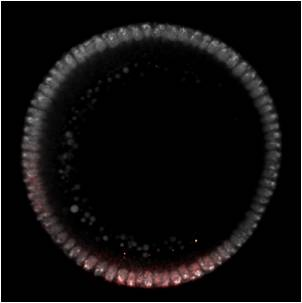
\includegraphics[width=0.1\textwidth]{dpERK_5min}};
        \node[right=0in of dpERK_5min] (mem_5min) {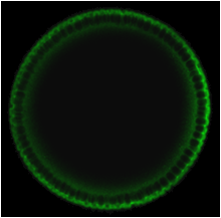
\includegraphics[width=0.1\textwidth]{membrane_5min}};
        \node[below=0.1in of dpERK_5min] (dpERK_20min) {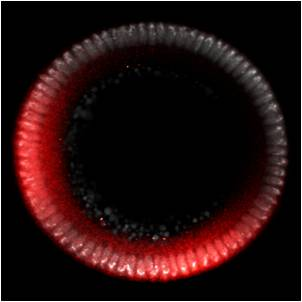
\includegraphics[width=0.1\textwidth]{dpERK_20min}};
        \node[right=0in of dpERK_20min] (mem_20min) {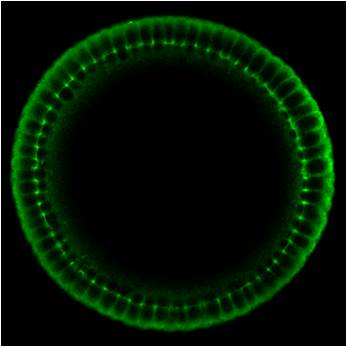
\includegraphics[width=0.1\textwidth]{membrane_20min}};
        \node[below=0.1in of dpERK_20min] (dpERK_45min) {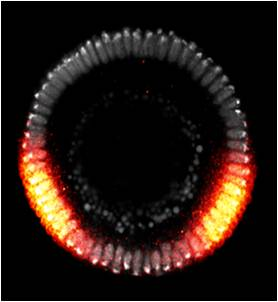
\includegraphics[width=0.1\textwidth]{dpERK_45min}};
        \node[right=0in of dpERK_45min] (mem_45min) {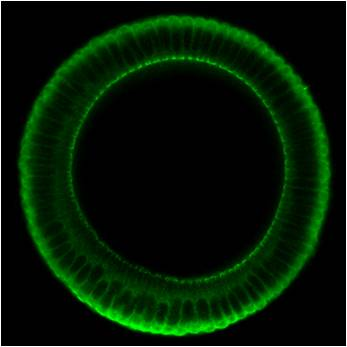
\includegraphics[width=0.1\textwidth]{membrane_45min}};
        \node[below=0.25in of $(dpERK_45min)!0.5!(mem_45min)$, text width=0.3\textwidth, align=center](text1) {{\small \em We stain each embryo for dpERK and membrane proteins \par}};
        \node[right=0.5in of mem_20min] (calibration) {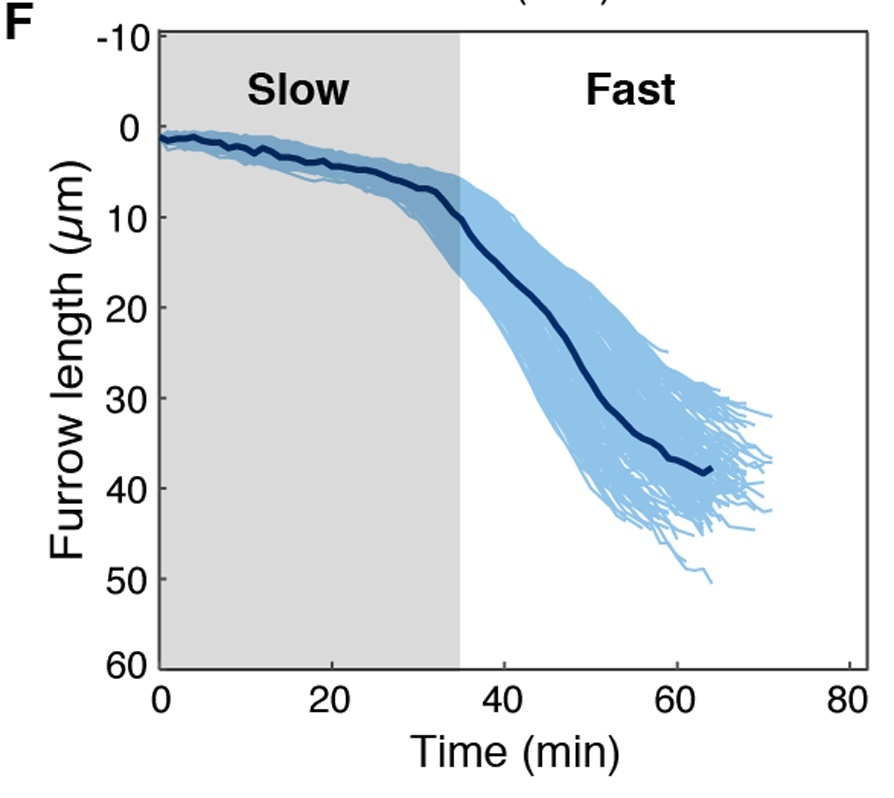
\includegraphics[width=0.3\textwidth]{calibration_curve}} edge[<-] (mem_5min) edge[<-] (mem_20min) edge[<-] (mem_45min);
        \node[below=0in of calibration, text width=0.3\textwidth, align=center](text2) {{\small \em The membrane thickness or ``furrow length'' is monotonic in time or age of the embryo \par}};
        \node[right=2.5in of mem_20min] (time_20) {20 minutes} edge[<-] (calibration);
        \node[right=2.5in of mem_5min] (time_5) {5 minutes} edge[<-] (calibration);
        \node[right=2.5in of mem_45min] (time_45) {45 minutes} edge[<-] (calibration);
        \node[below=0in of time_45, text width=0.25\textwidth, align=center](text2) {{\small \em We can calculate the age of each embryo from the membrane thickness \par}};
    \end{tikzpicture}

We can therefore assess the quality of our orderings by plotting the embedding coordinate as a function of membrane thickness; this should be one--to--one.
\end{frame}


\begin{frame}{Comparing Scattering Transform Ordering to Membrane Thickness}

	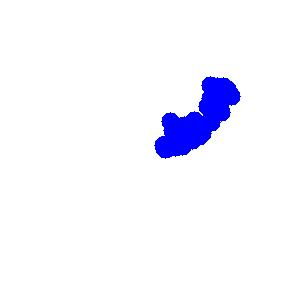
\includegraphics[width=0.5\textwidth]{DMAPS_scat_time_corr}

	The DMAPS embedding coordinate using the scattering transform (which we use to order the data) is well--correlated with the membrane thickness (which is known to be monotonic in time).
	
\end{frame}

\begin{frame}{Ordering Two--Dimensional Membrane Images}

We could also use our techniques (e.g. scattering transform + DMAPS) to temporally order the fluorescent {\em membrane} images.

\foreach \i in {15, 19, 30, 42, 45, 10, 36, 46, 47, 51, 27, 24, 28, 48, 38, 52, 34, 20, 50, 17, 6, 22, 16, 39, 33, 21, 2, 41, 9, 29, 14, 4, 8, 35, 31, 3, 40, 44, 13, 7, 18, 32, 11, 43, 25, 49, 5, 26, 23, 37, 12} {	
	\includegraphics[width=0.05\textwidth]{membrane_scat_raw_all_\i}} 
    
    	\centering
    {\Large $\downarrow$}
    
	\foreach \i in {15, 19, 30, 42, 45, 10, 36, 46, 47, 51, 27, 24, 28, 48, 38, 52, 34, 20, 50, 17, 6, 22, 16, 39, 33, 21, 2, 41, 9, 29, 14, 4, 8, 35, 31, 3, 40, 44, 13, 7, 18, 32, 11, 43, 25, 49, 5, 26, 23, 37, 12} {	
	\includegraphics[width=0.05\textwidth]{membrane_scat_all_\i}}  
	
	Because we are interested only in the membrane thickness, we first apply an edge--detection filter to the images.
	
	\end{frame}

\begin{frame}{Ordering of Two-Dimensional Membrane Images}
	
%	{\small
%	\begin{itemize}
%		\item 	We can also use the scattering transform coefficient with DMAPS to order the membrane images themselves.   
%		\item Because we are interested in the membrane thickness, we first run an edge detection algorithm \footcite{canny1986computational} to extract the membrane edges from the images.
%		\item We then use the Euclidean distance between the scattering transform coefficients of the edge detected images in a DMAPS calculation
%	\end{itemize}
%	\par}

%    \centering
%    \begin{tikzpicture}
%    	\node[anchor=south west] (image) {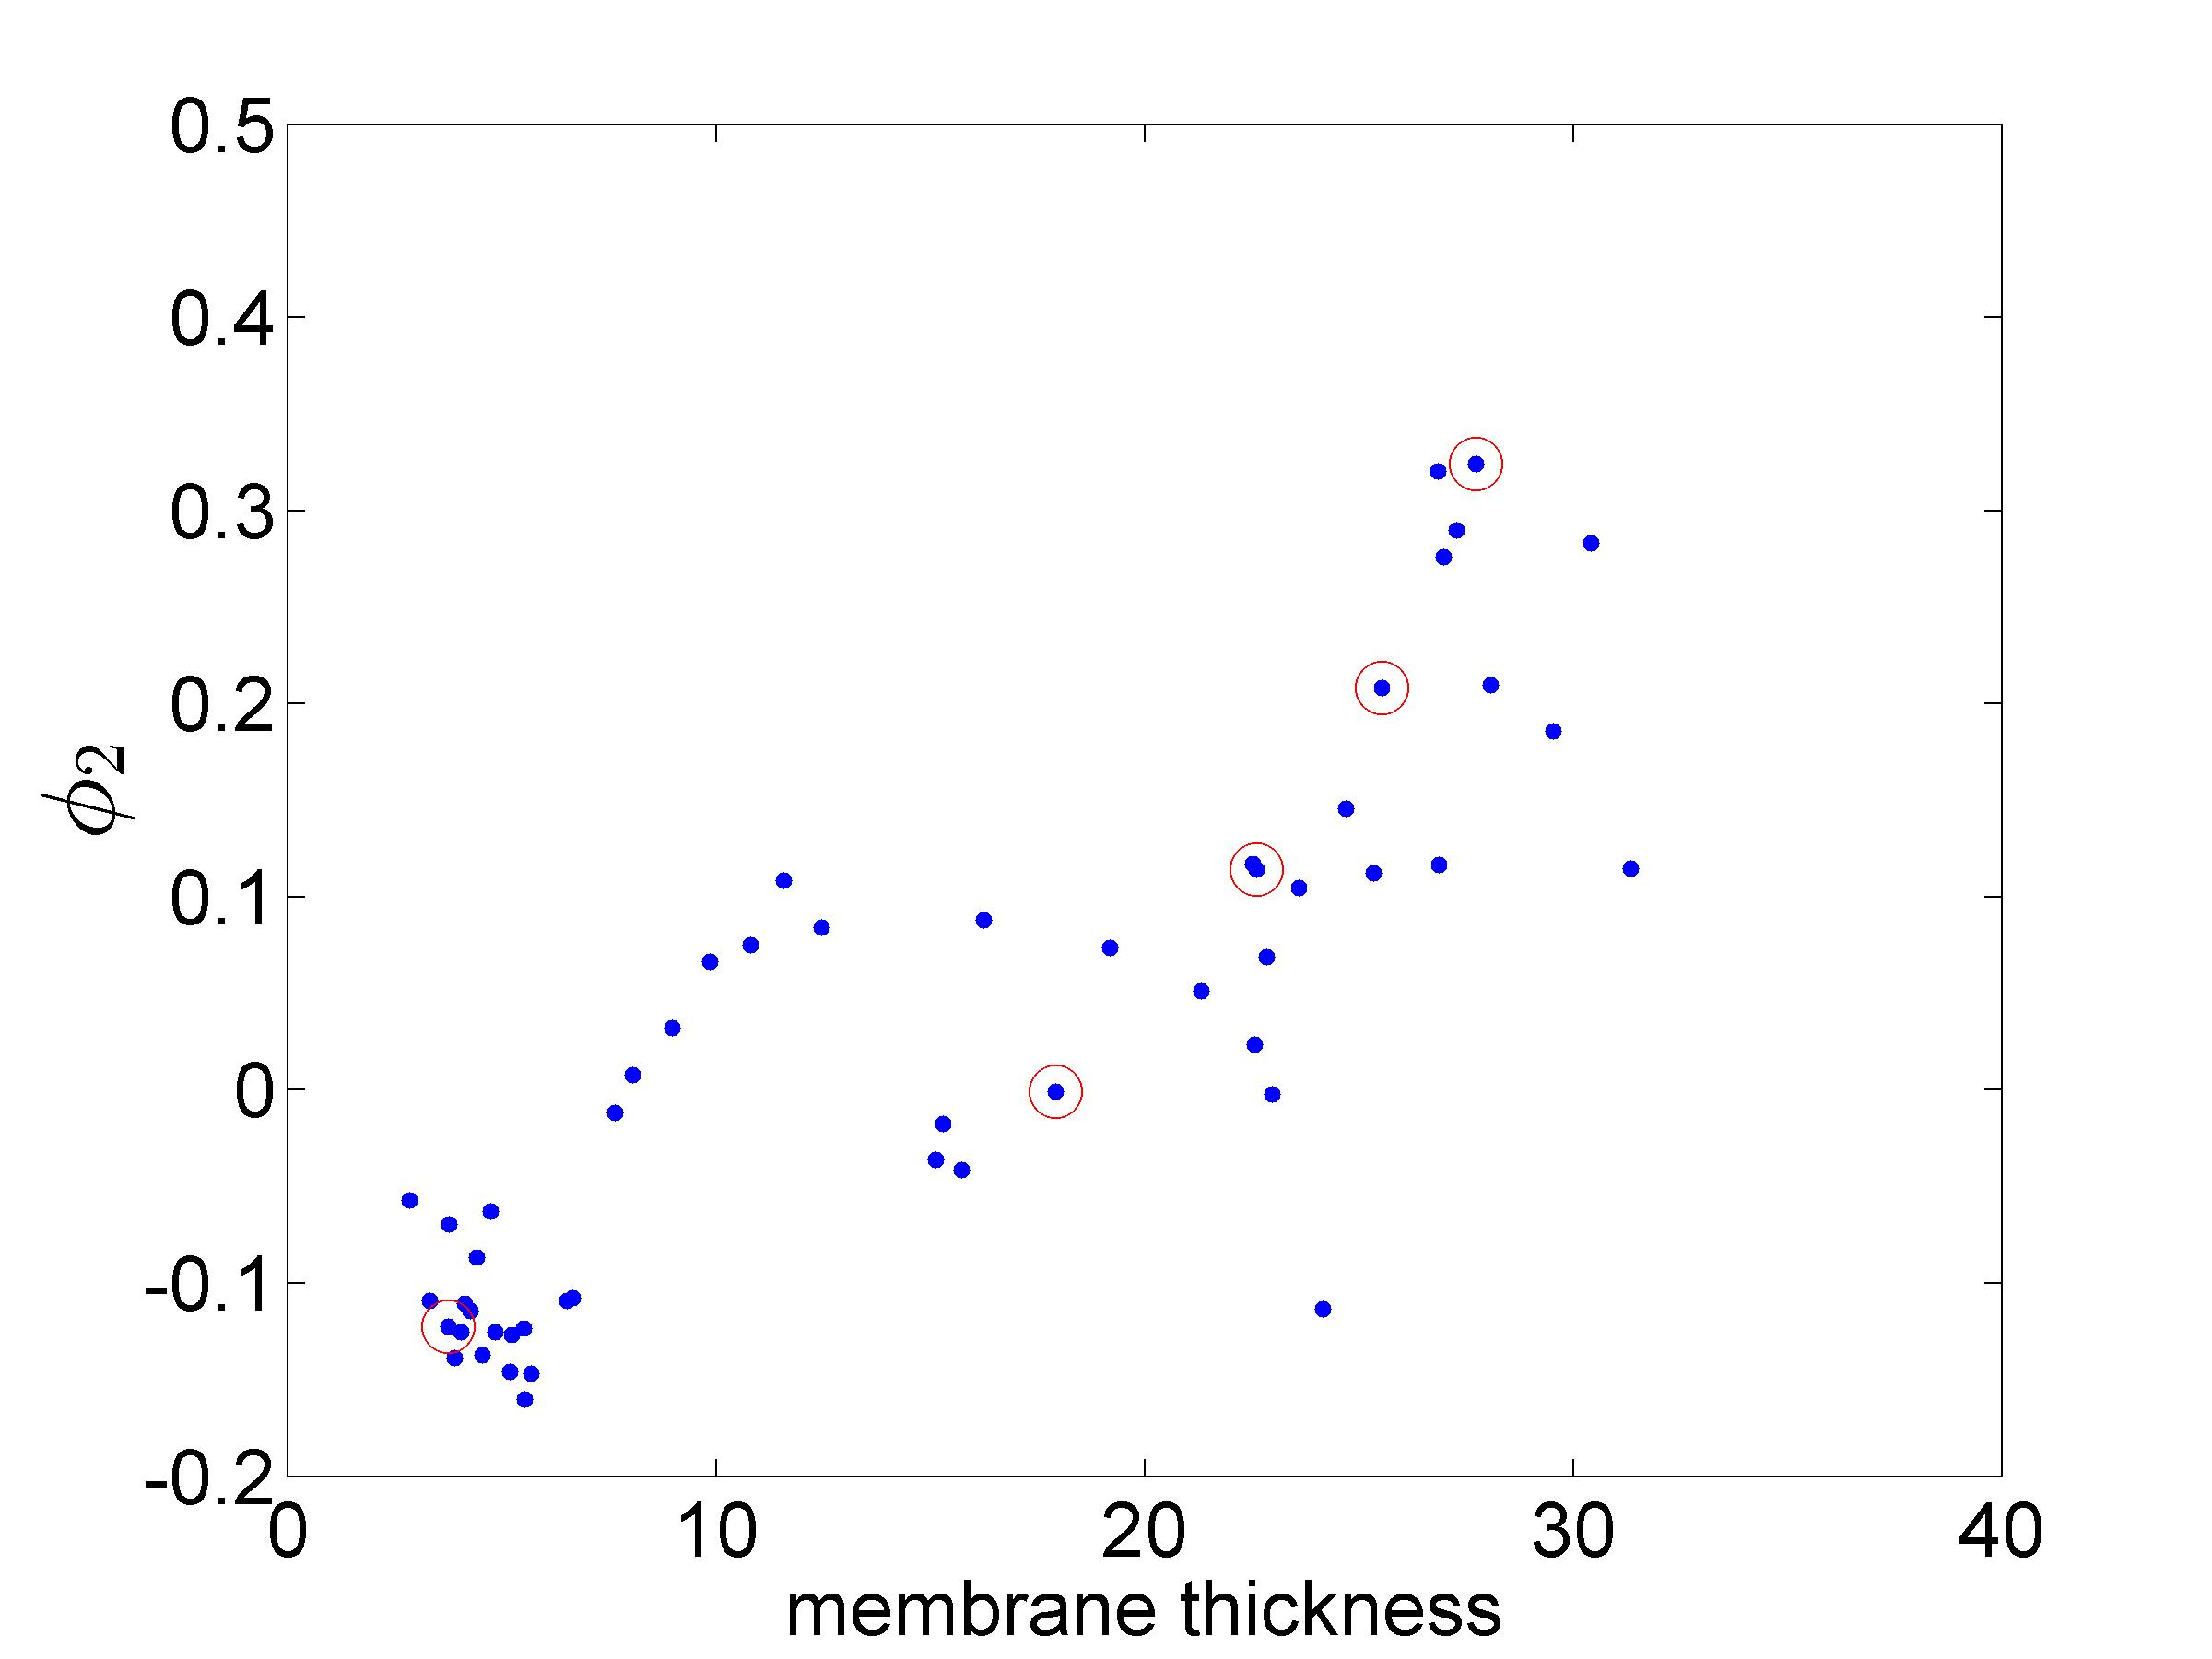
\includegraphics[width=0.4\textwidth]{DMAPS_membrane_scat_time_corr2}};
%    	\begin{scope}[x={(image.south east)},y={(image.north west)}]
%    	%\draw[help lines,xstep=.05,ystep=.05] (0,0) grid (1,1);
%    	\node(x1) at (0.23,0.23) {};
%    	\node(x2) at (0.50,0.38) {};
%    	\node(x3) at (0.57,0.51) {};
%    	\node(x4) at (0.61,0.62) {};
%    	\node(x5) at (0.64,0.74) {};
%    	\end{scope}
%    	\node[below=0.2in of image](fig3) {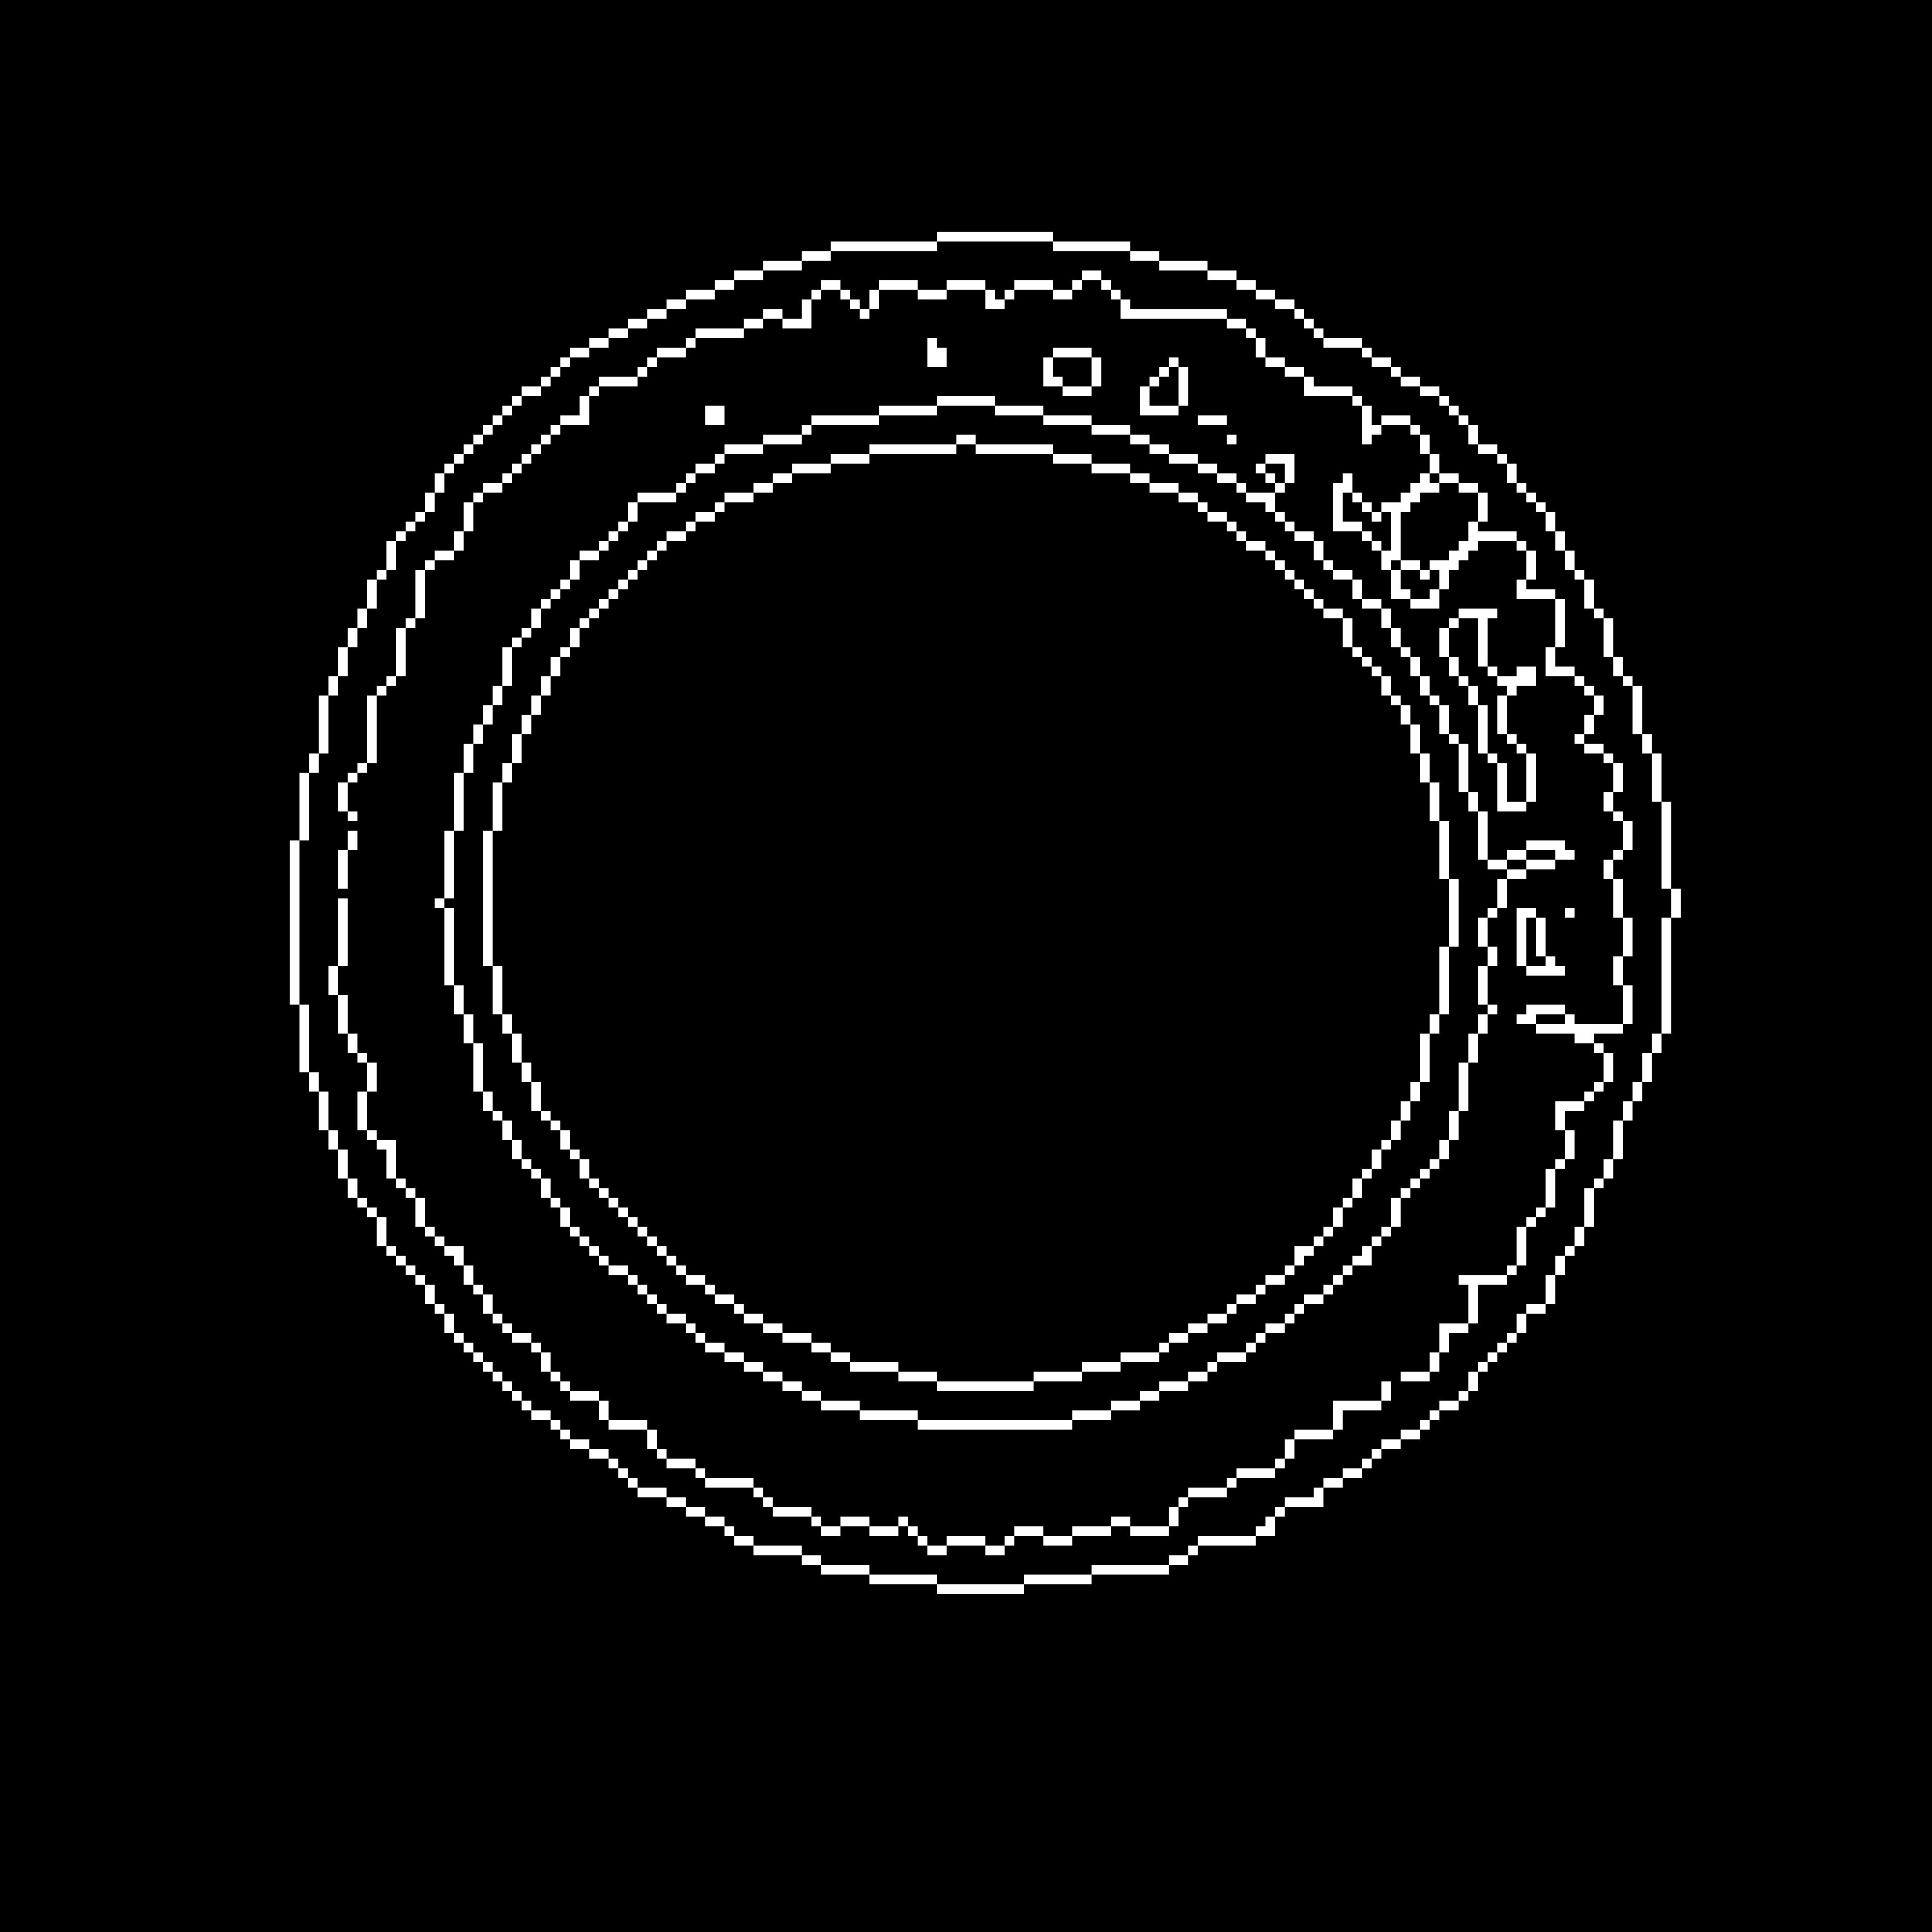
\includegraphics[width=0.1\textwidth]{membrane_scat_3}};		
%    	\node[left=0.1in of fig3](fig2) {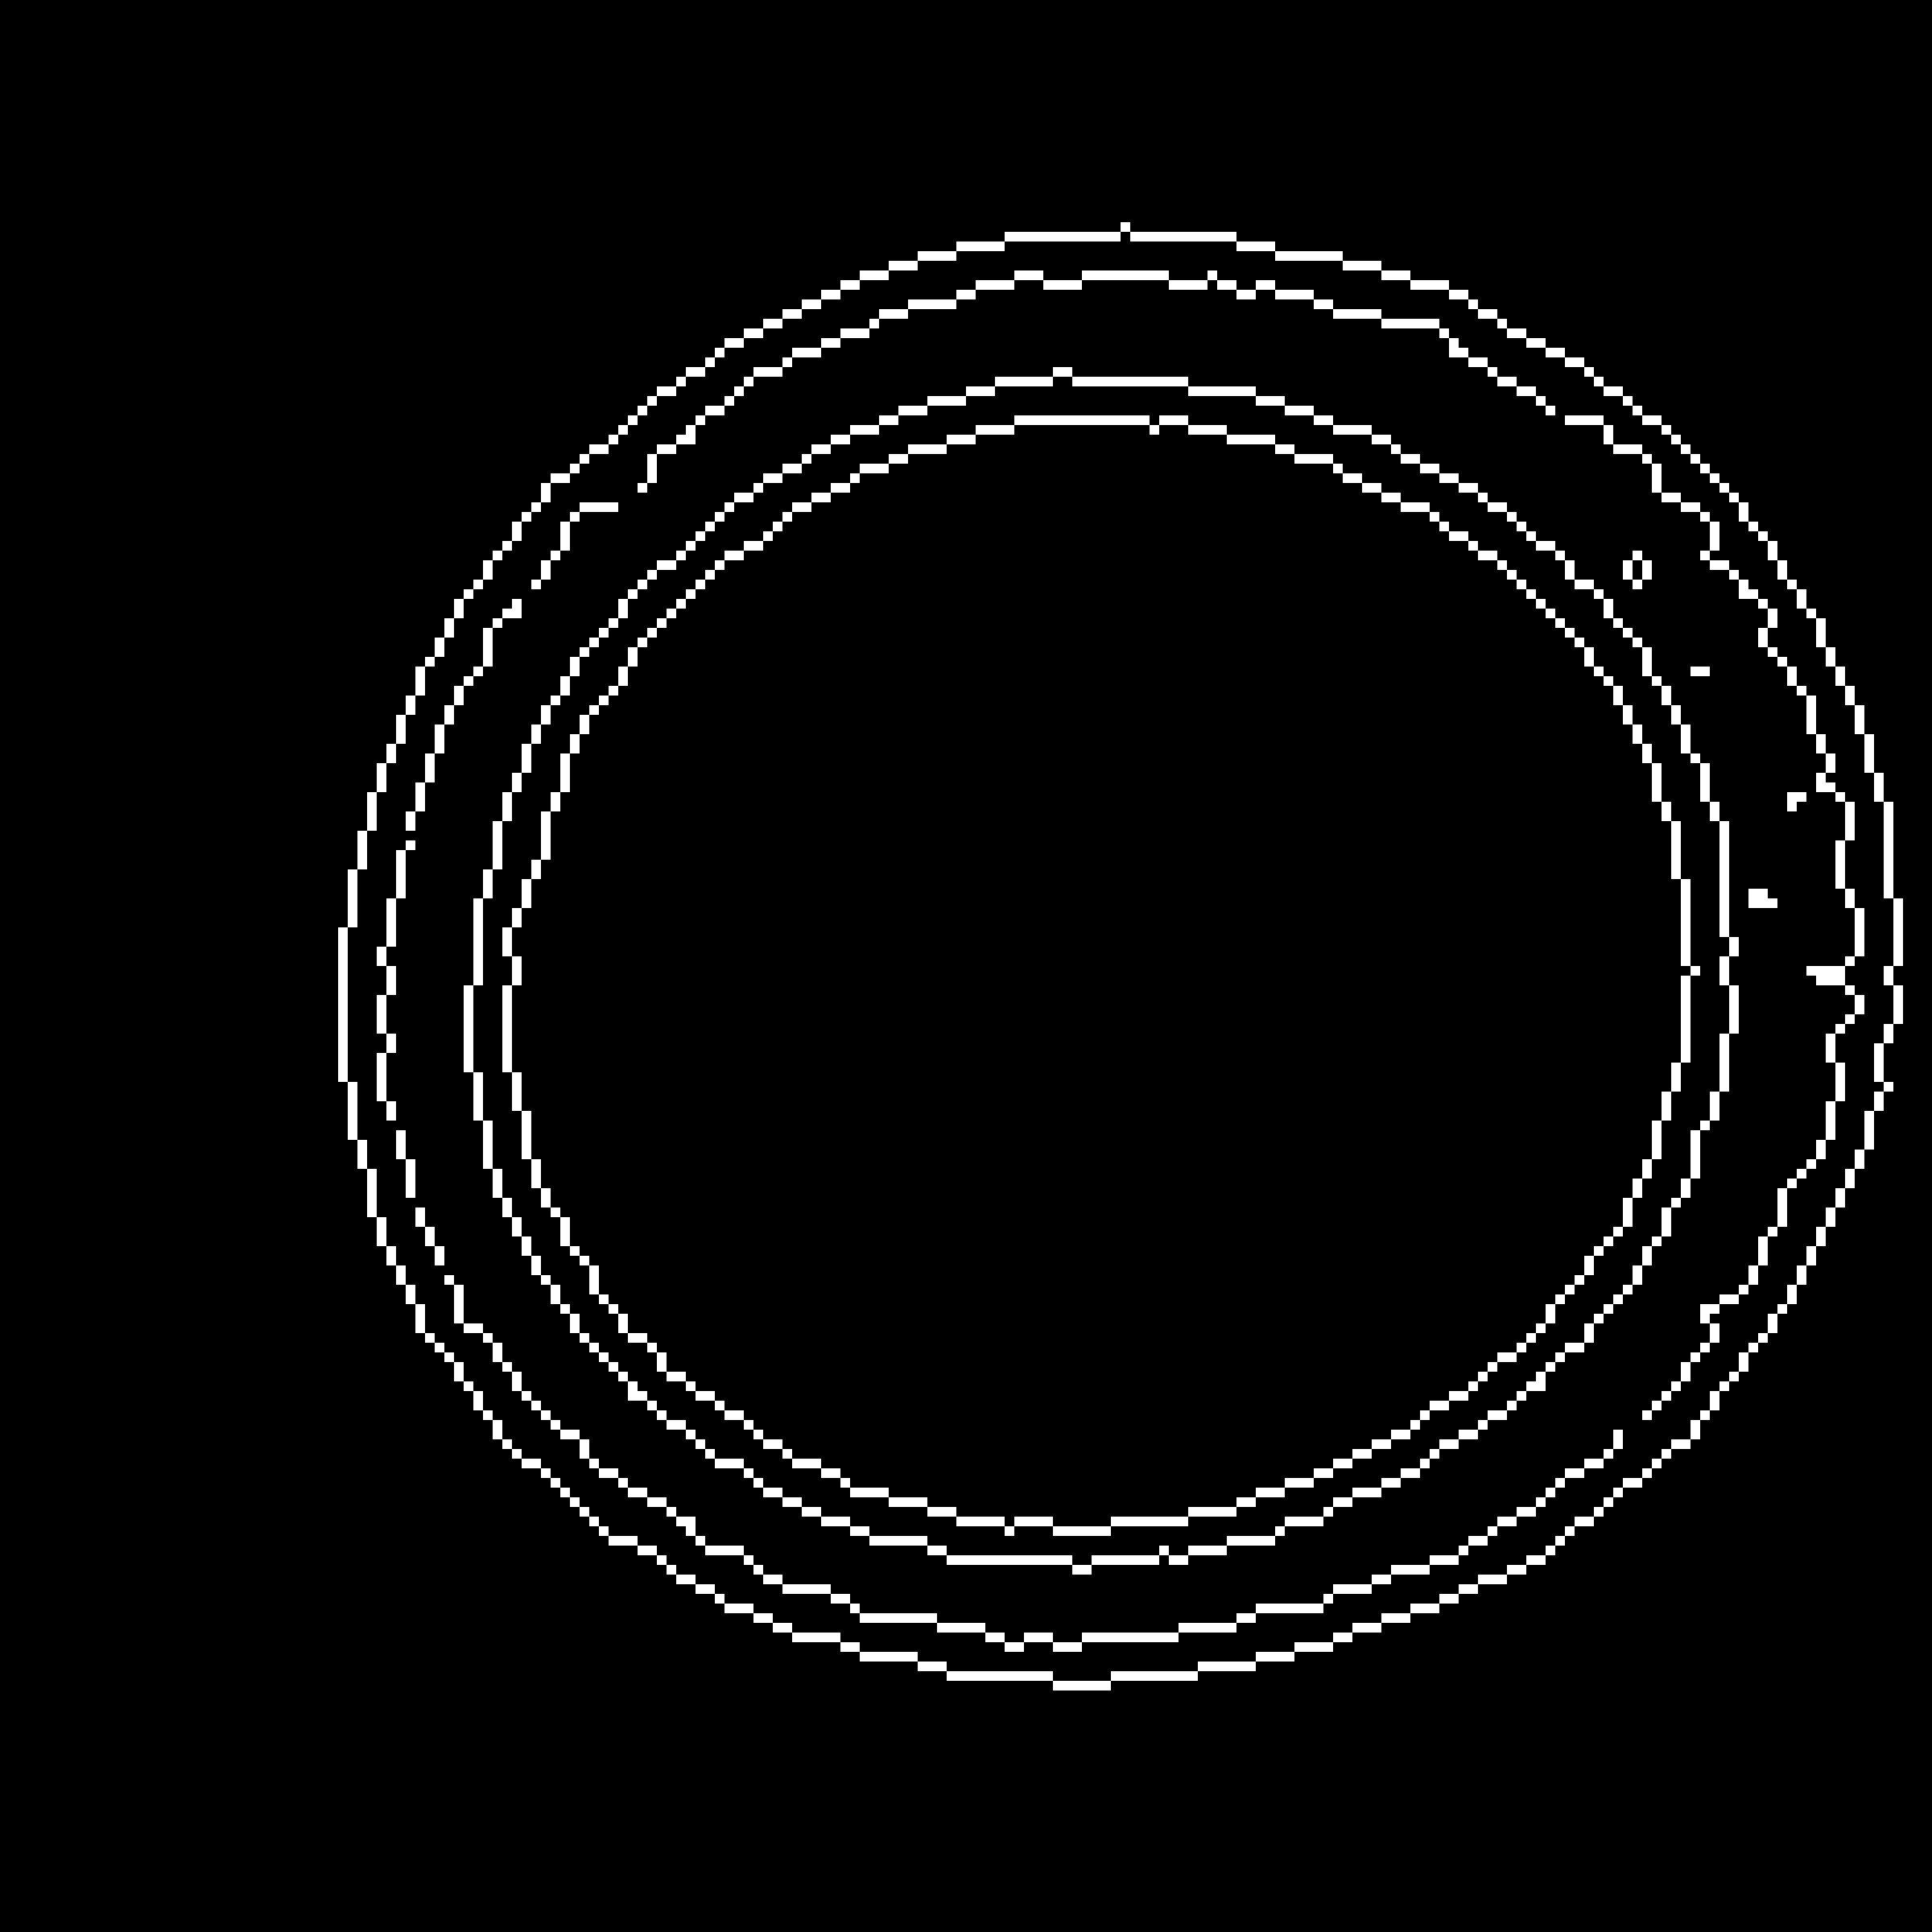
\includegraphics[width=0.1\textwidth]{membrane_scat_2}};
%    	\node[left=0.1in of fig2](fig1) {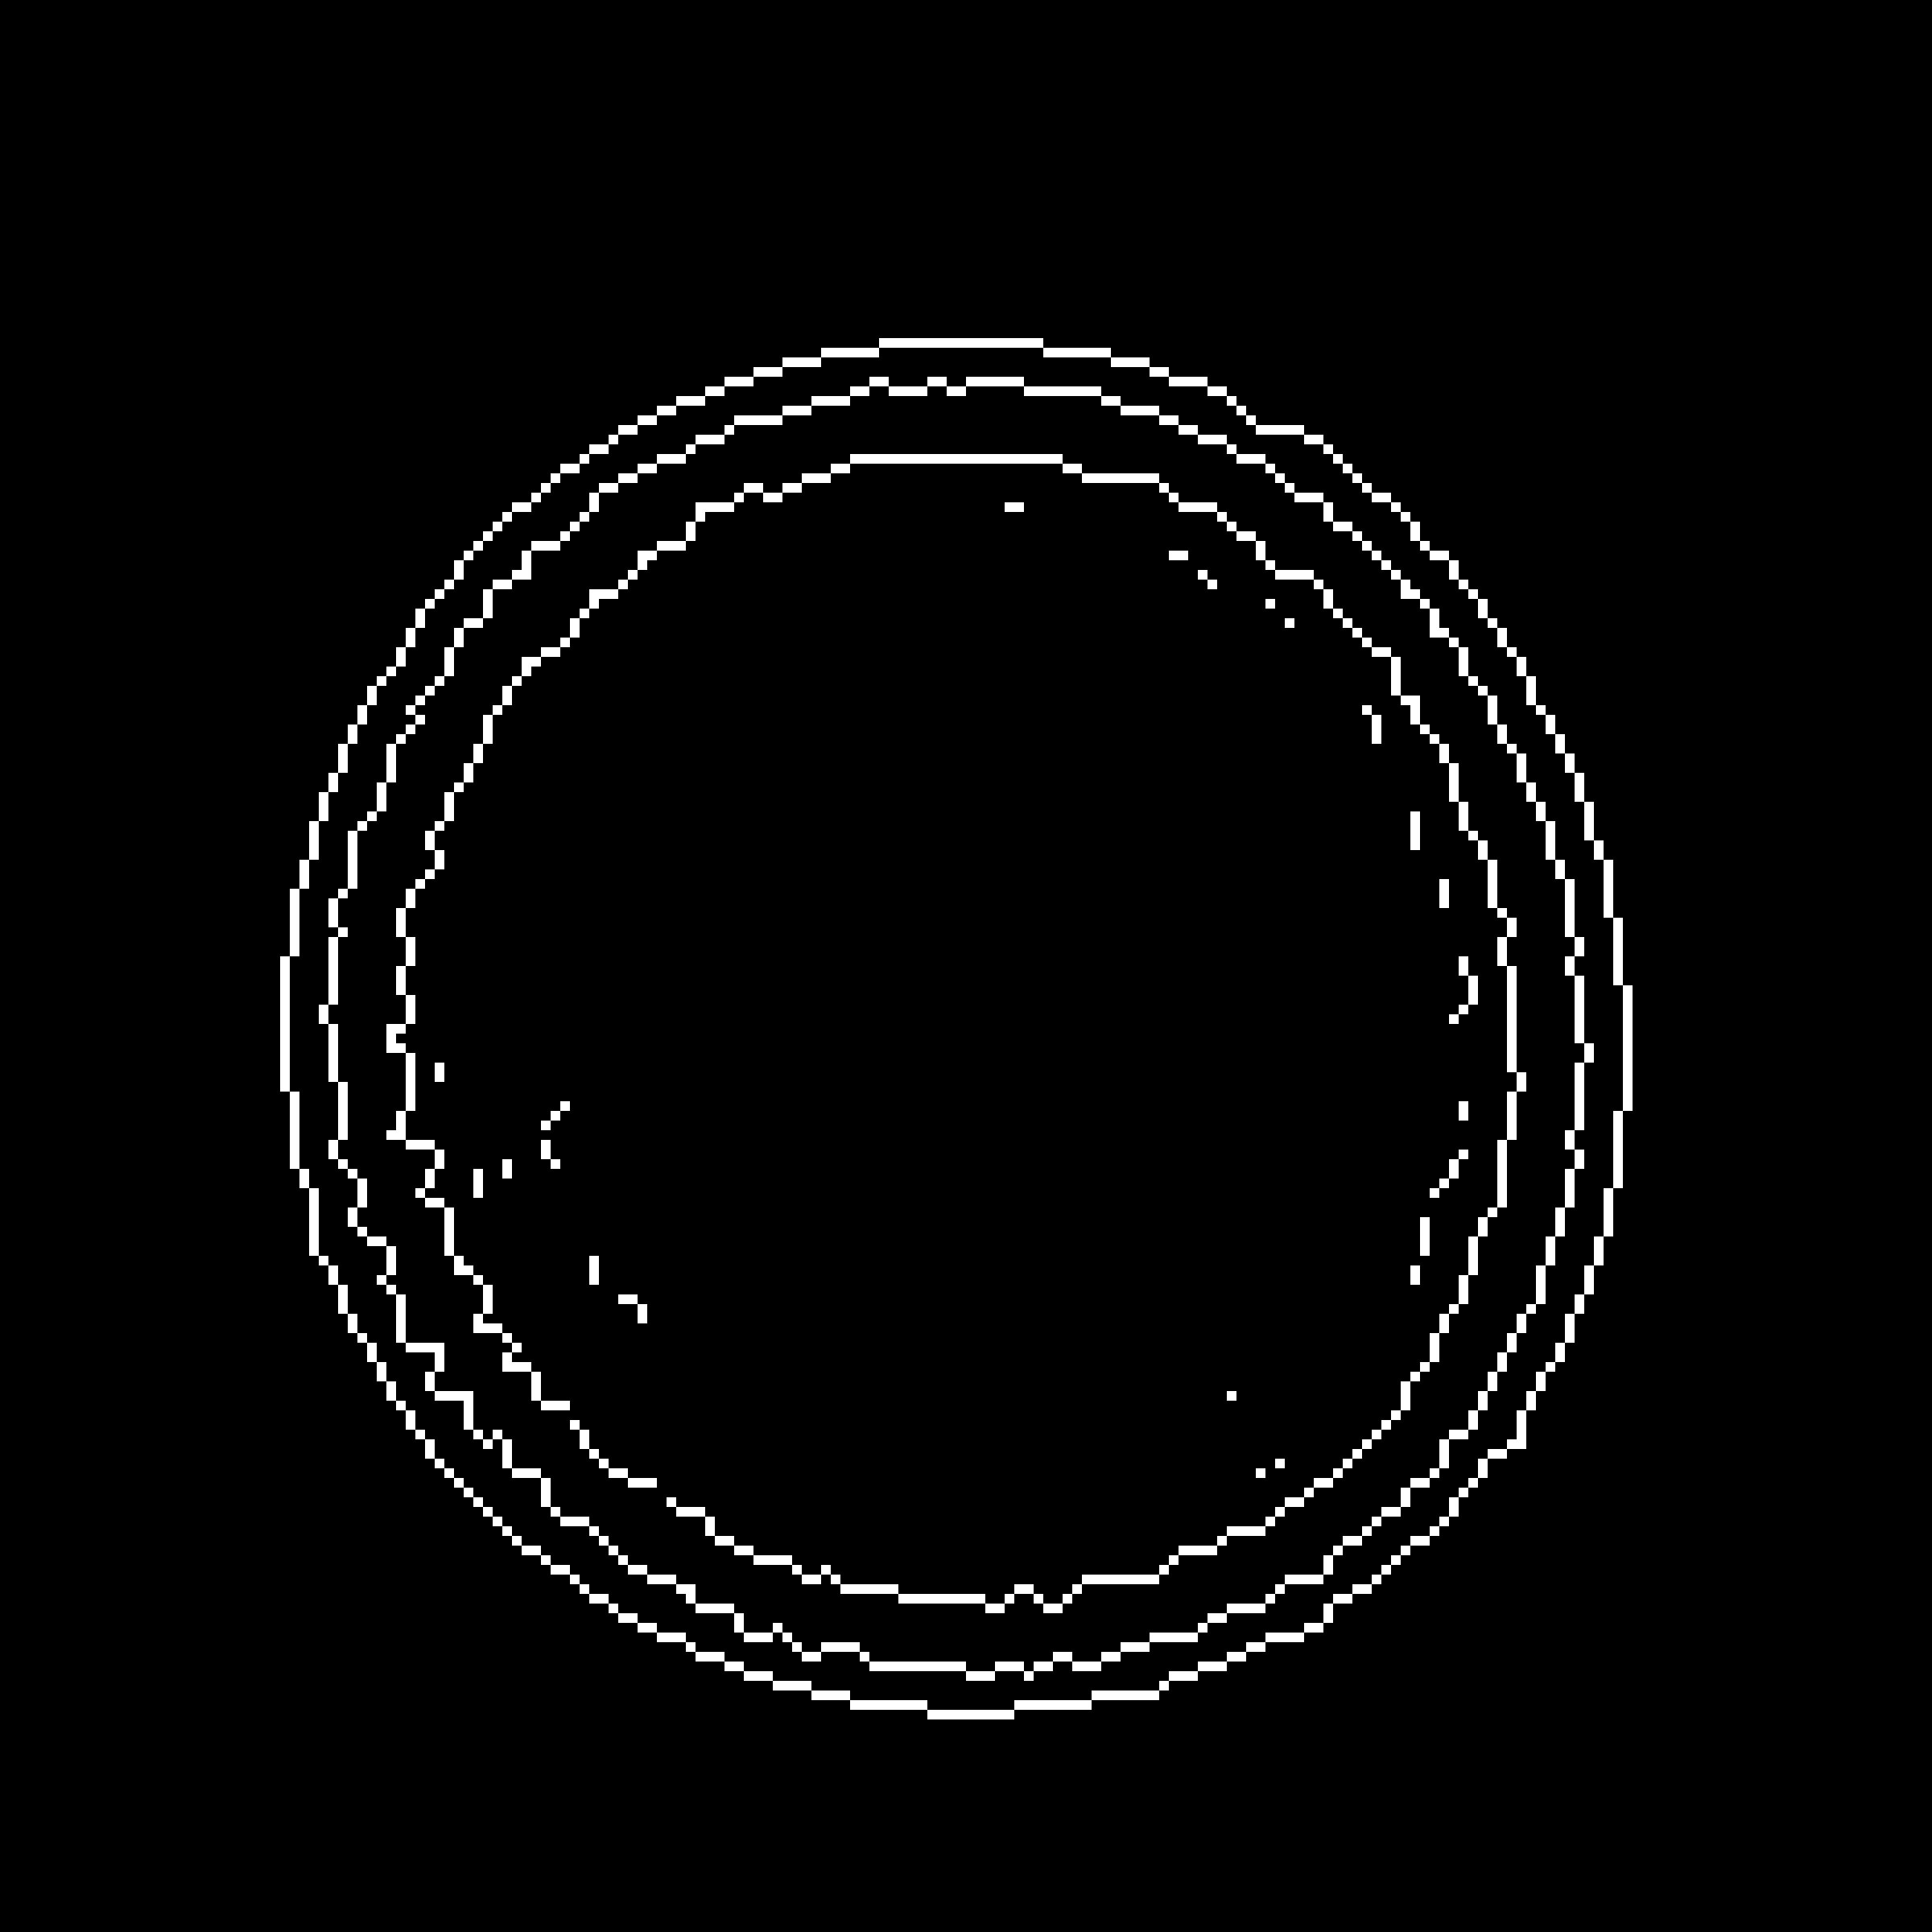
\includegraphics[width=0.1\textwidth]{membrane_scat_1}};	
%    	\node[right=0.1in of fig3](fig4) {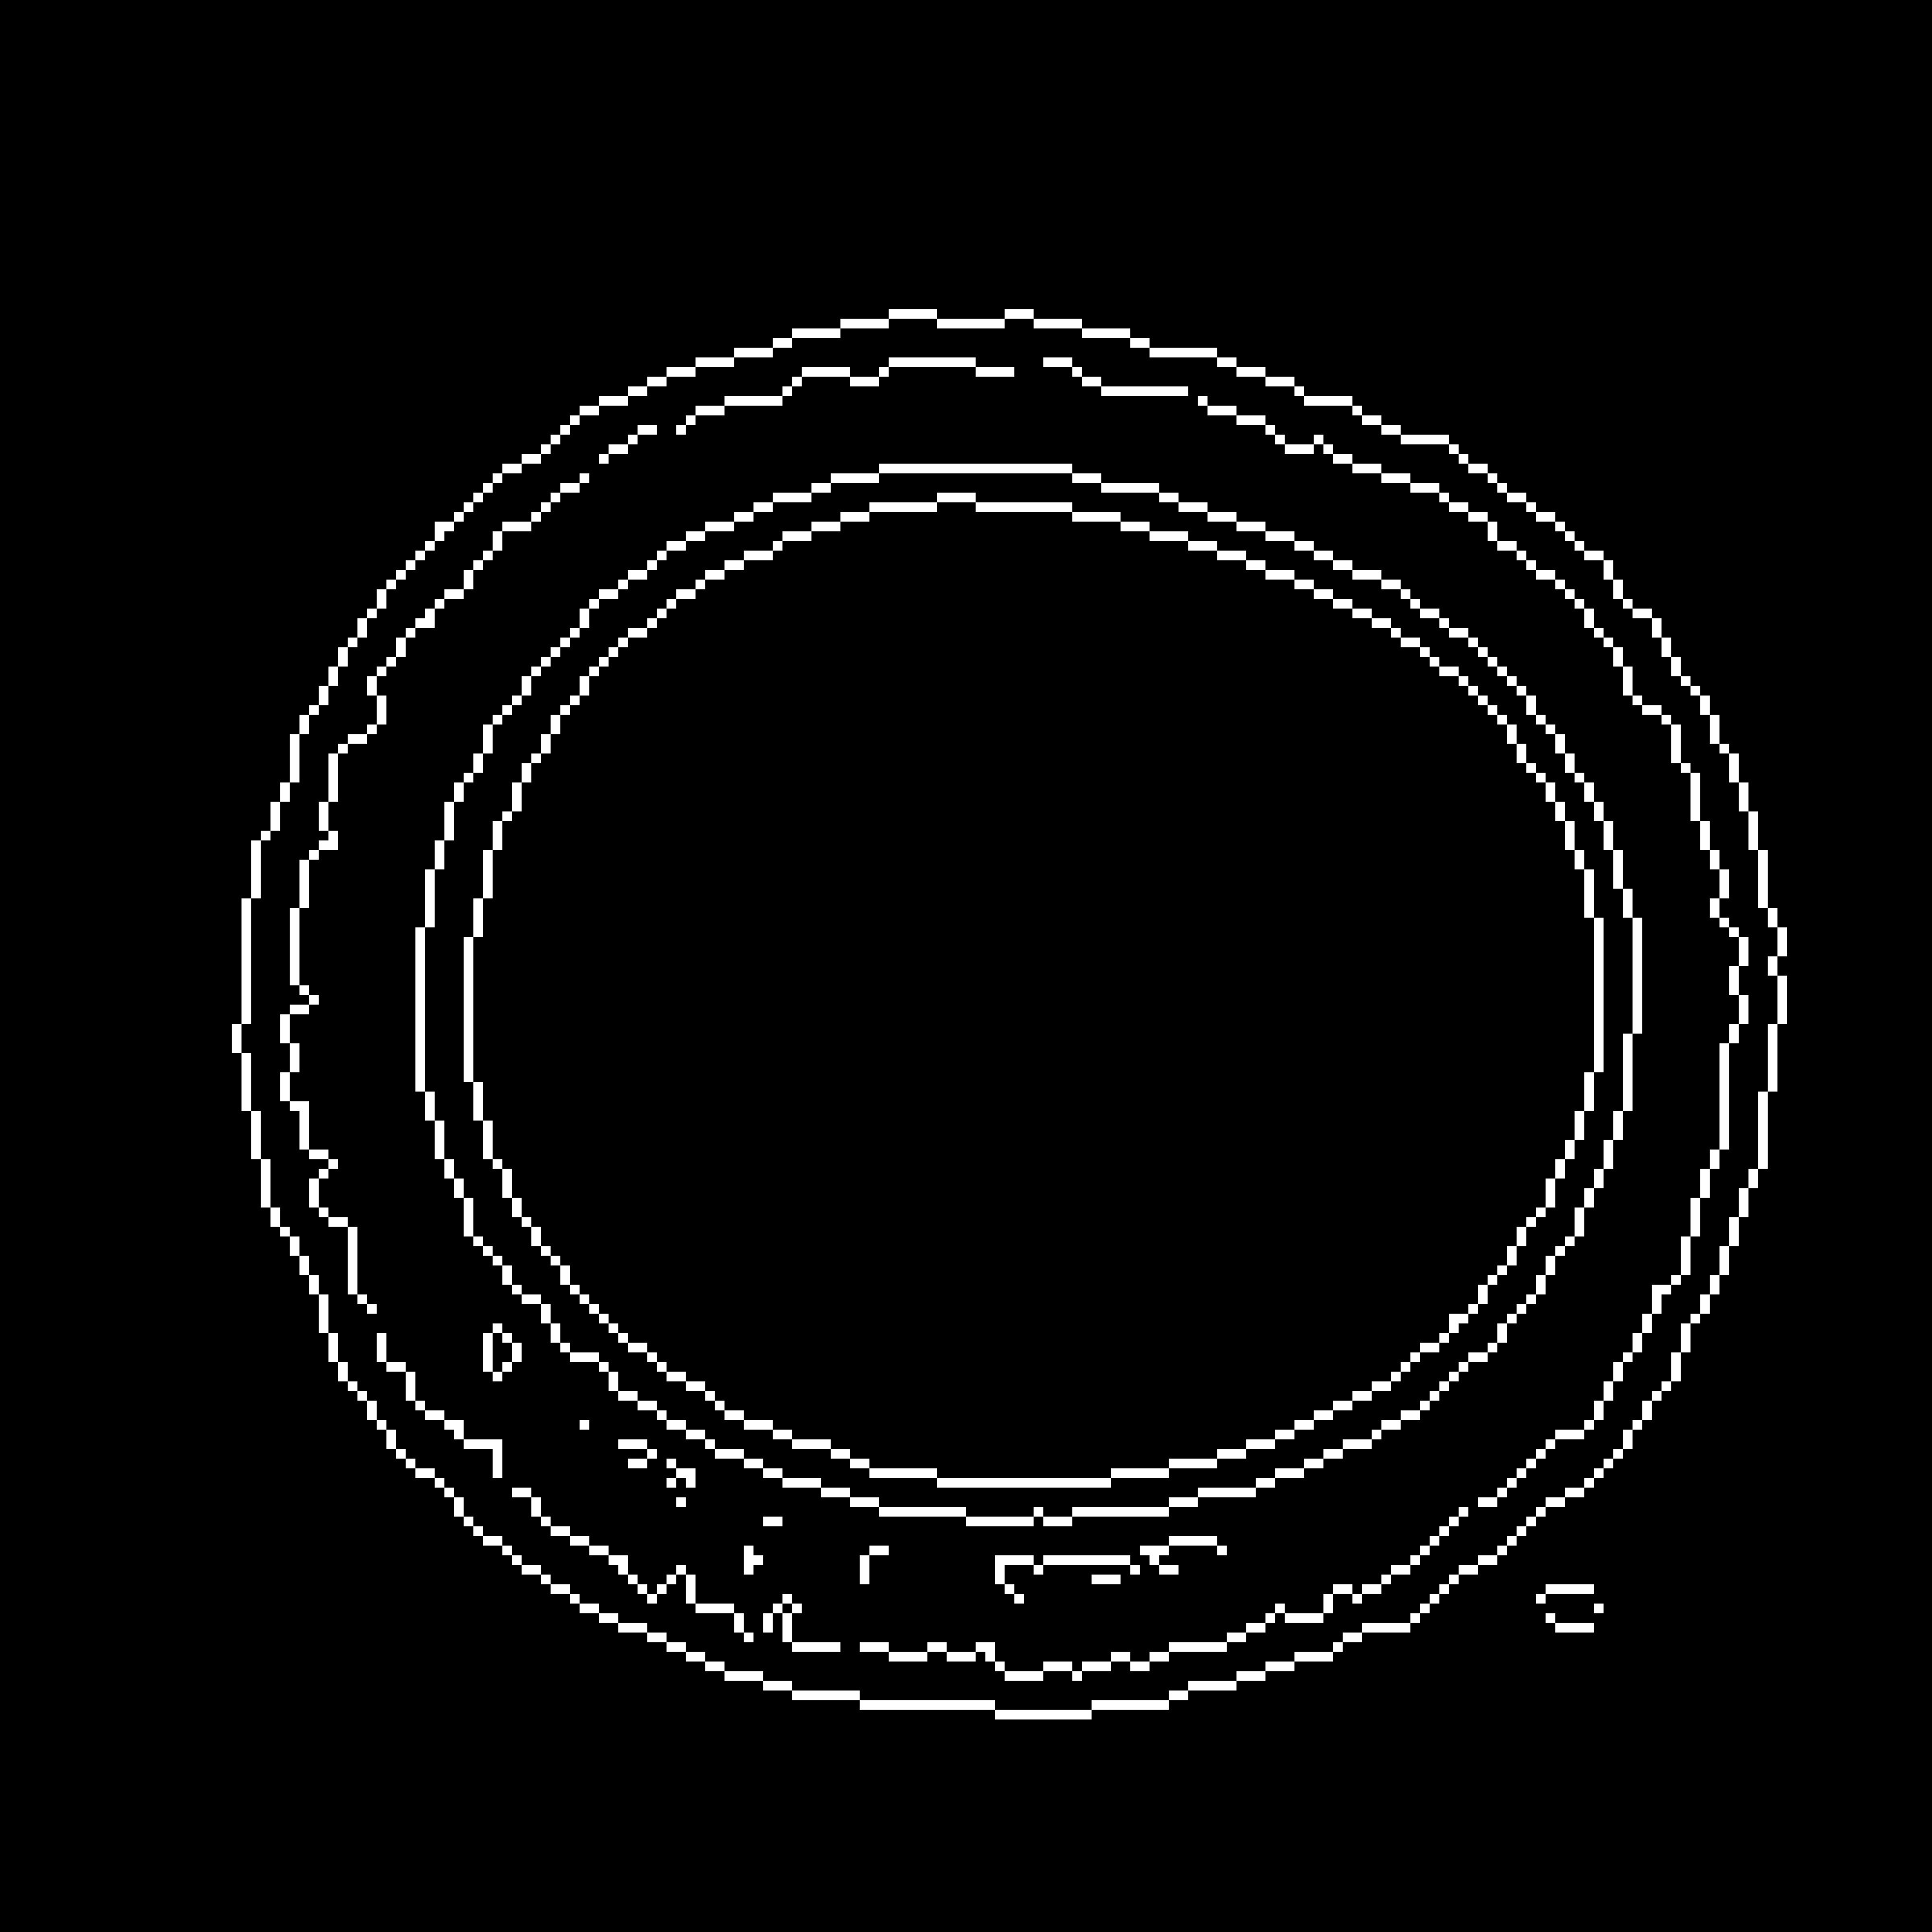
\includegraphics[width=0.1\textwidth]{membrane_scat_4}};					
%    	\node[right=0.1in of fig4](fig5) {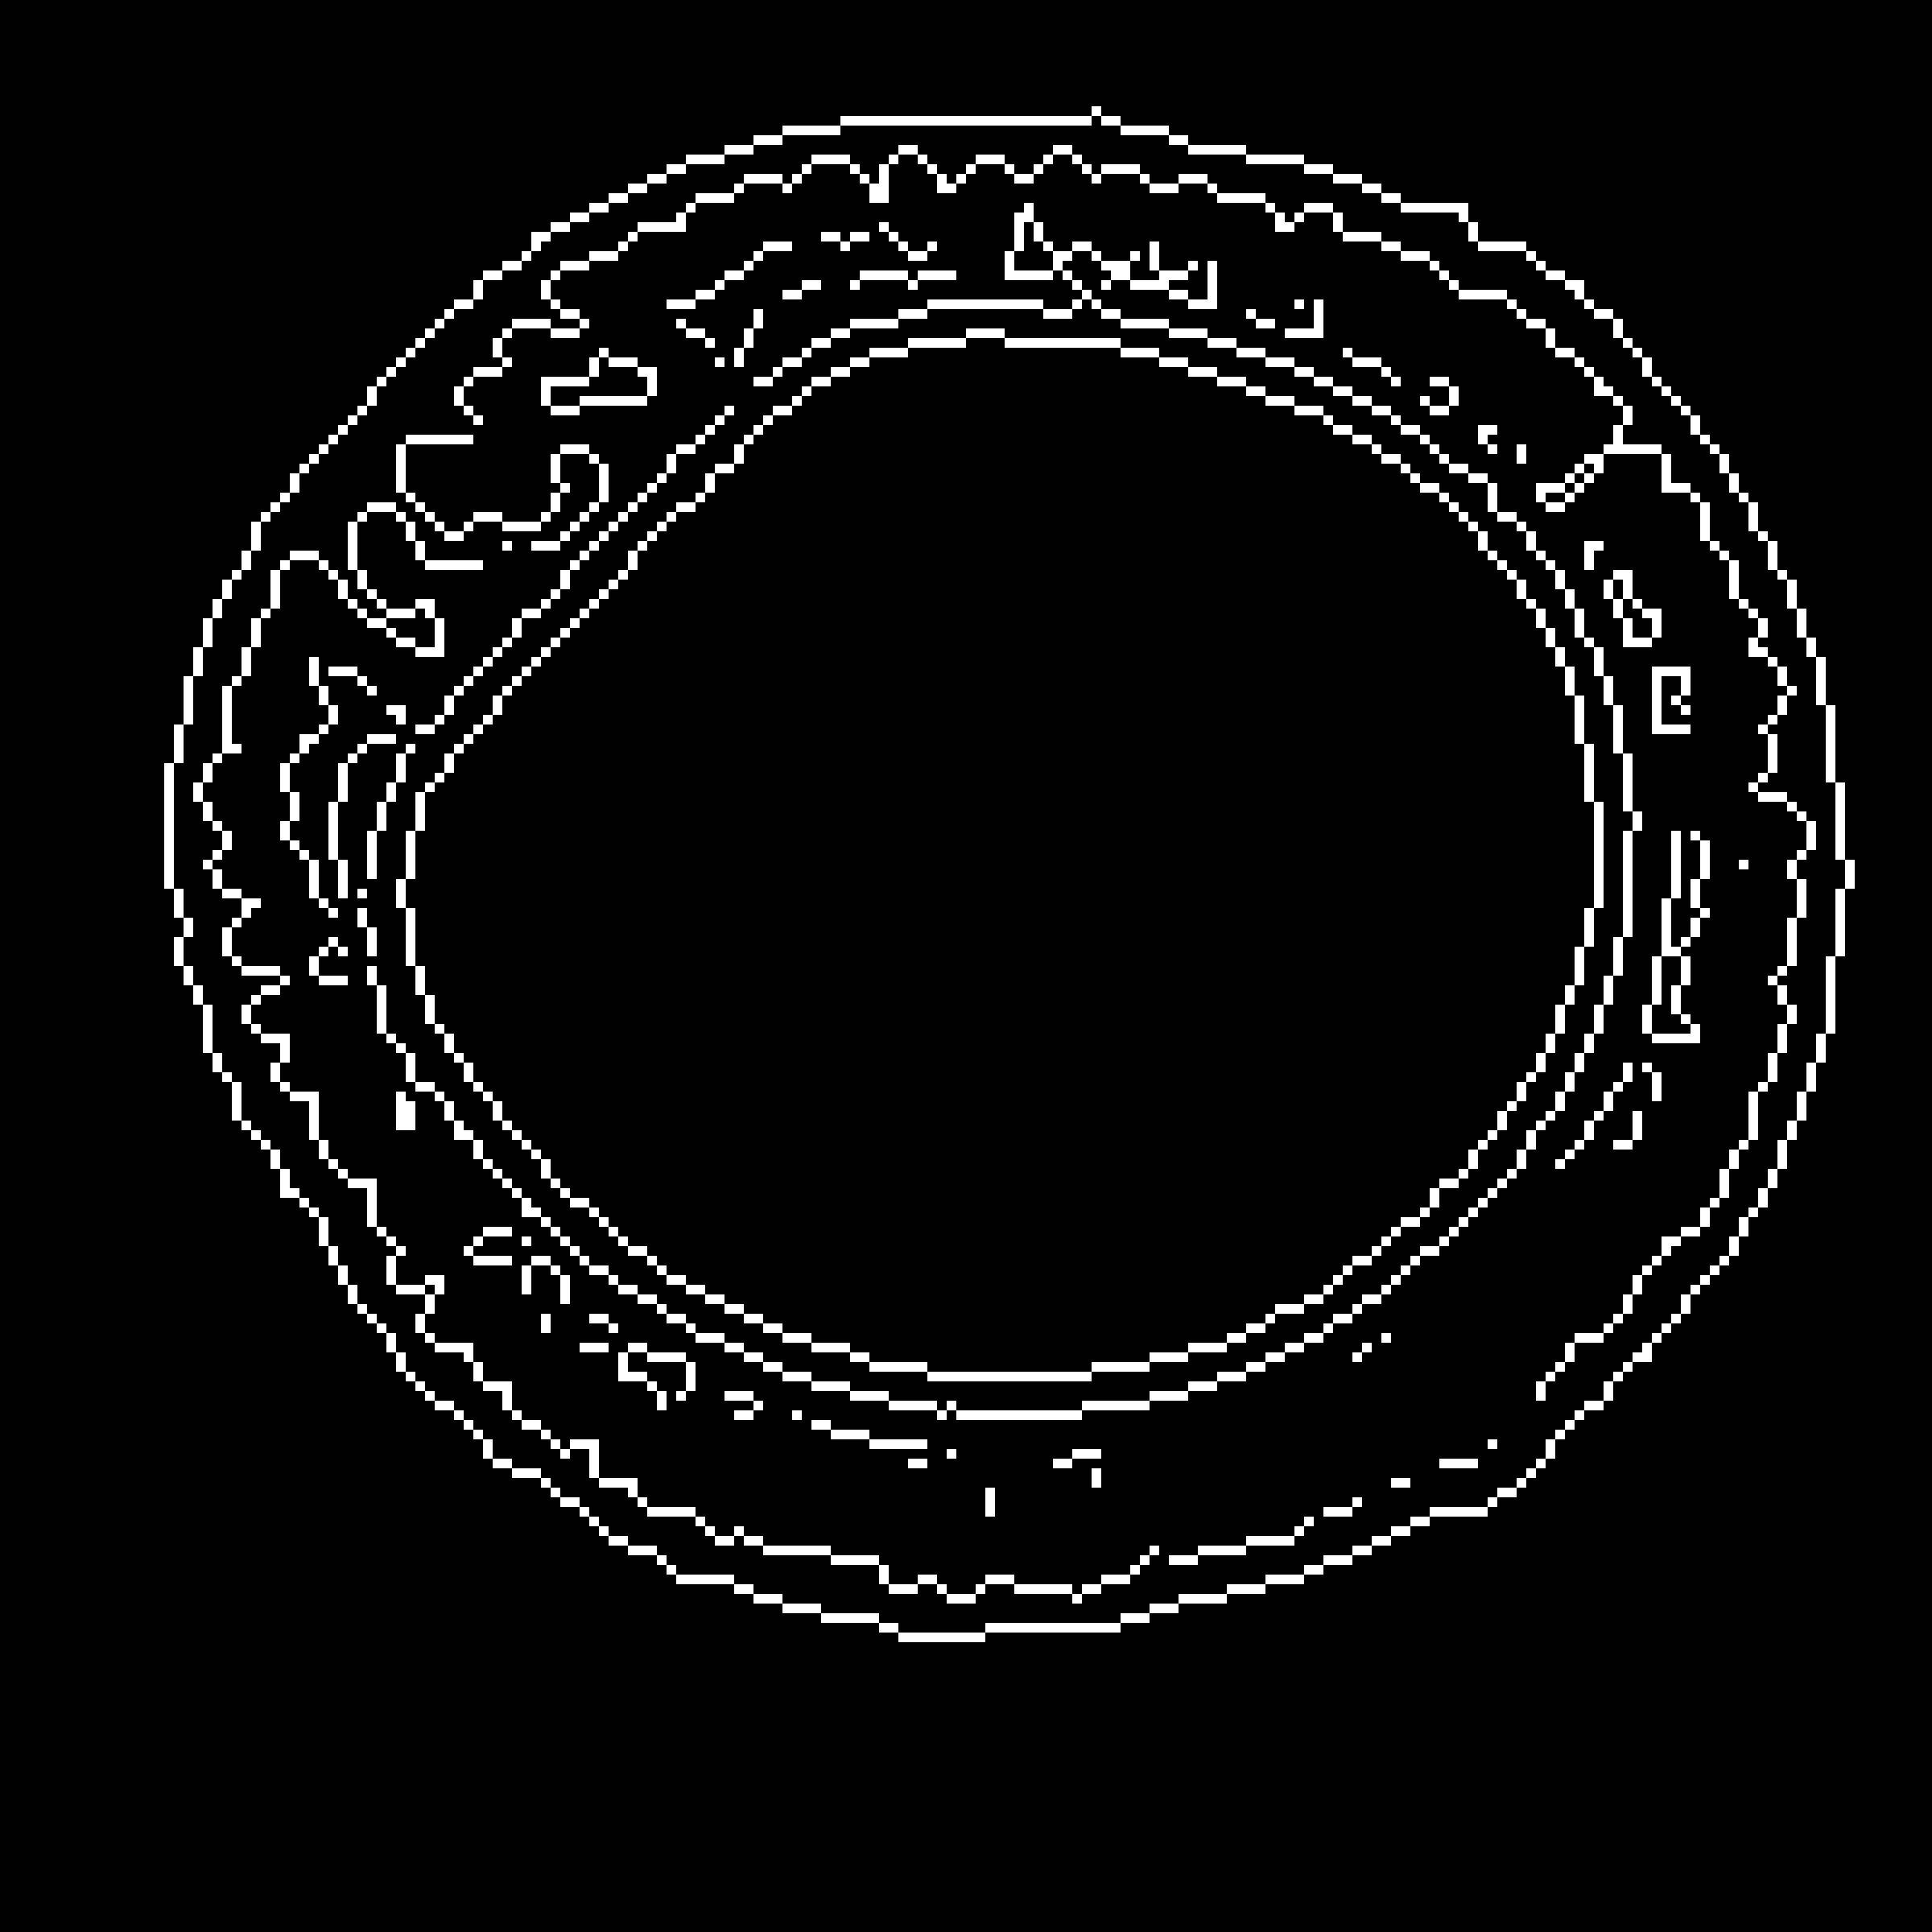
\includegraphics[width=0.1\textwidth]{membrane_scat_5}};
%    	\node[below=0.02in of fig3](fig3b) {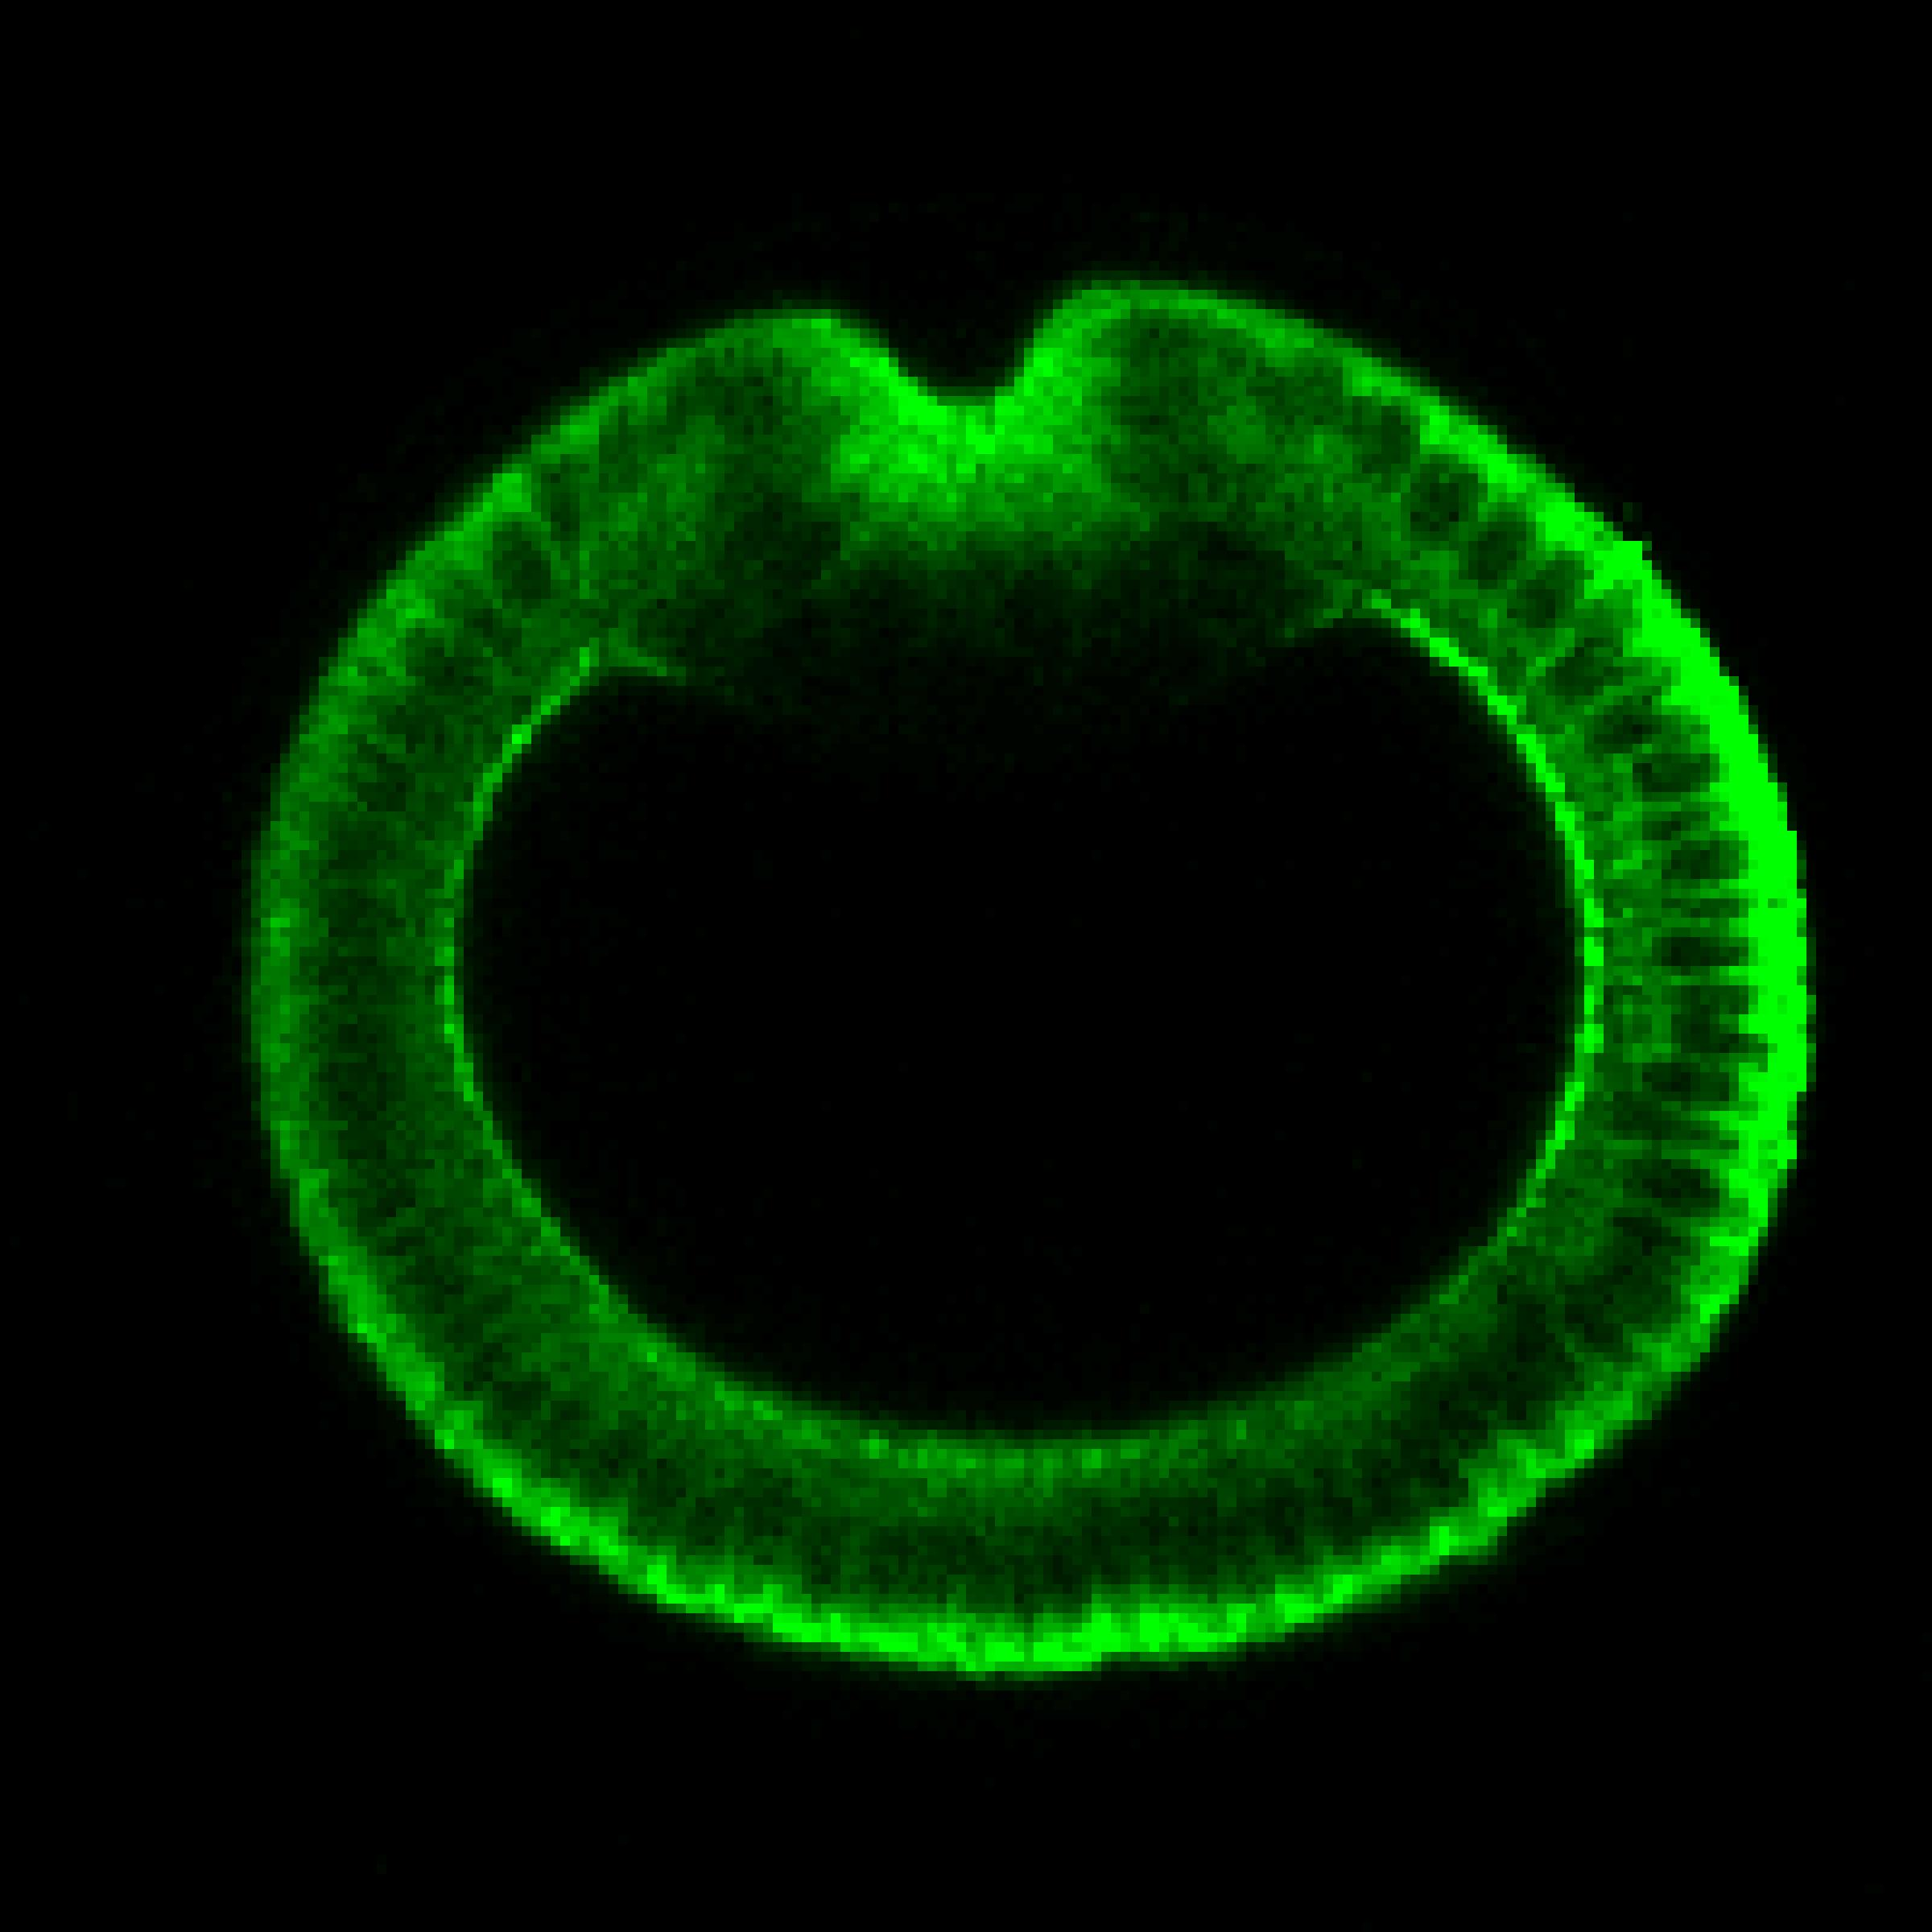
\includegraphics[width=0.1\textwidth]{membrane_scat_raw_3}};		
%    	\node[left=0.1in of fig3b](fig2b) {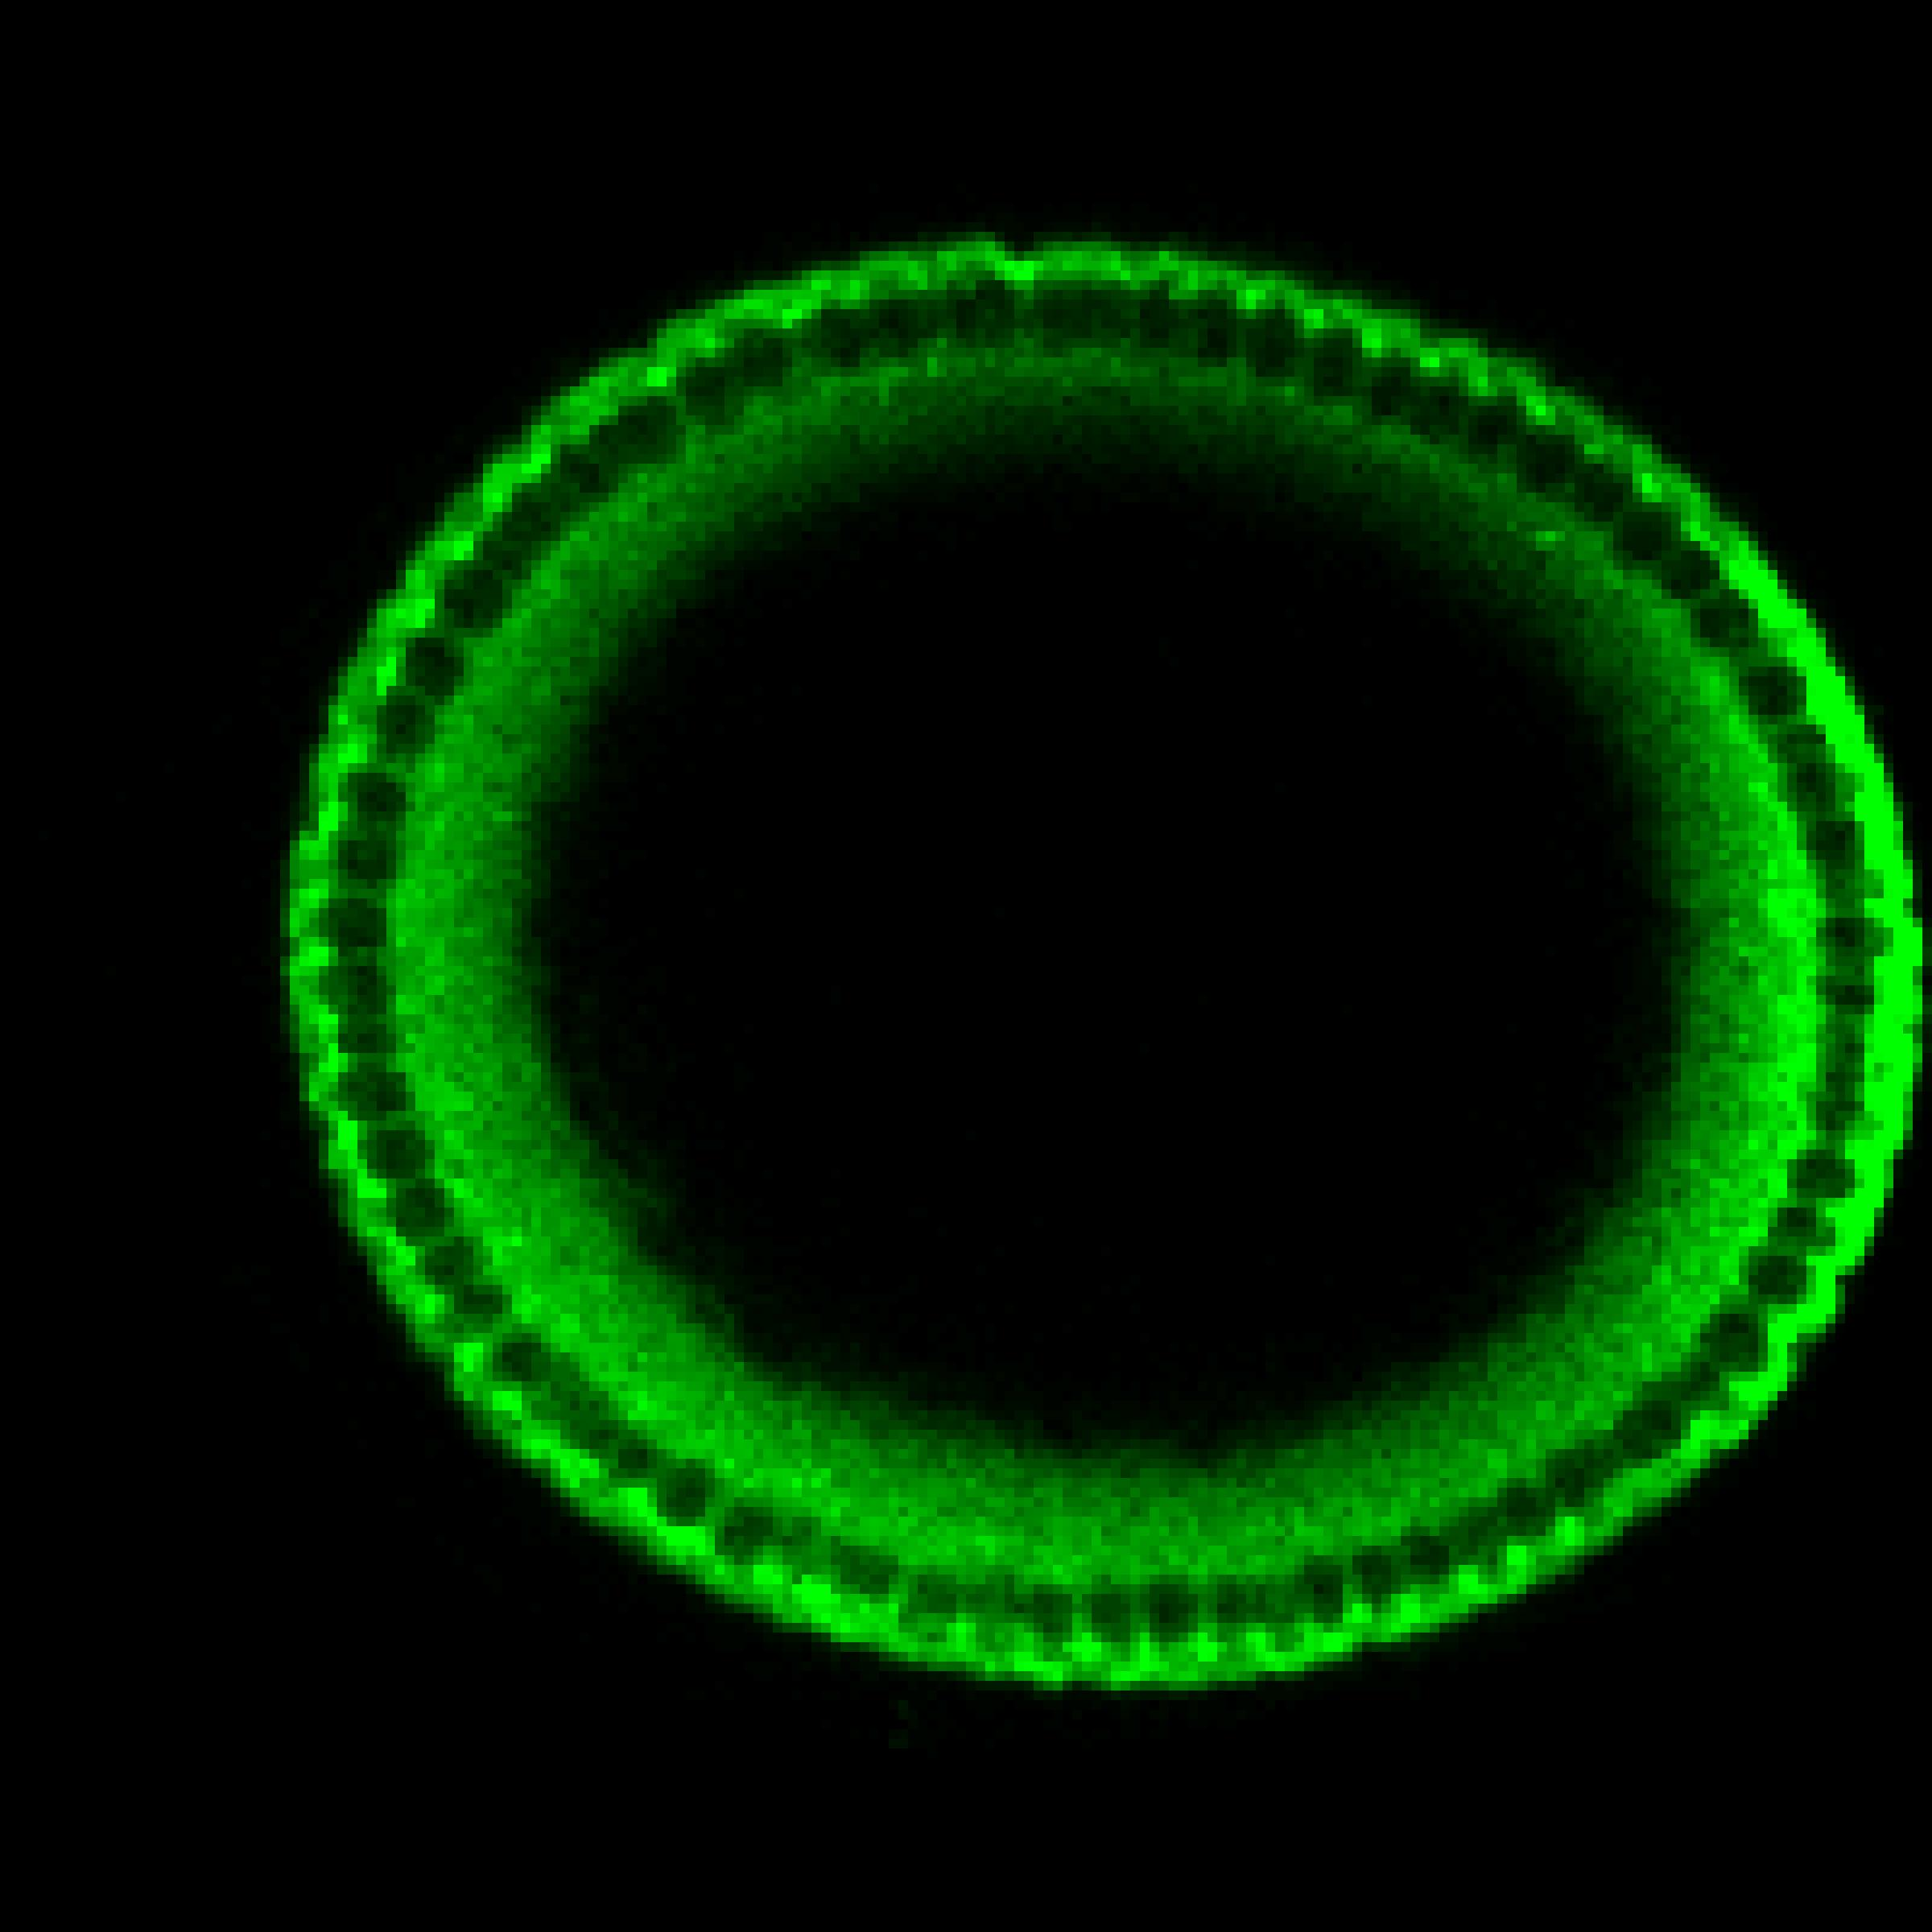
\includegraphics[width=0.1\textwidth]{membrane_scat_raw_2}};
%    	\node[left=0.1in of fig2b](fig1b) {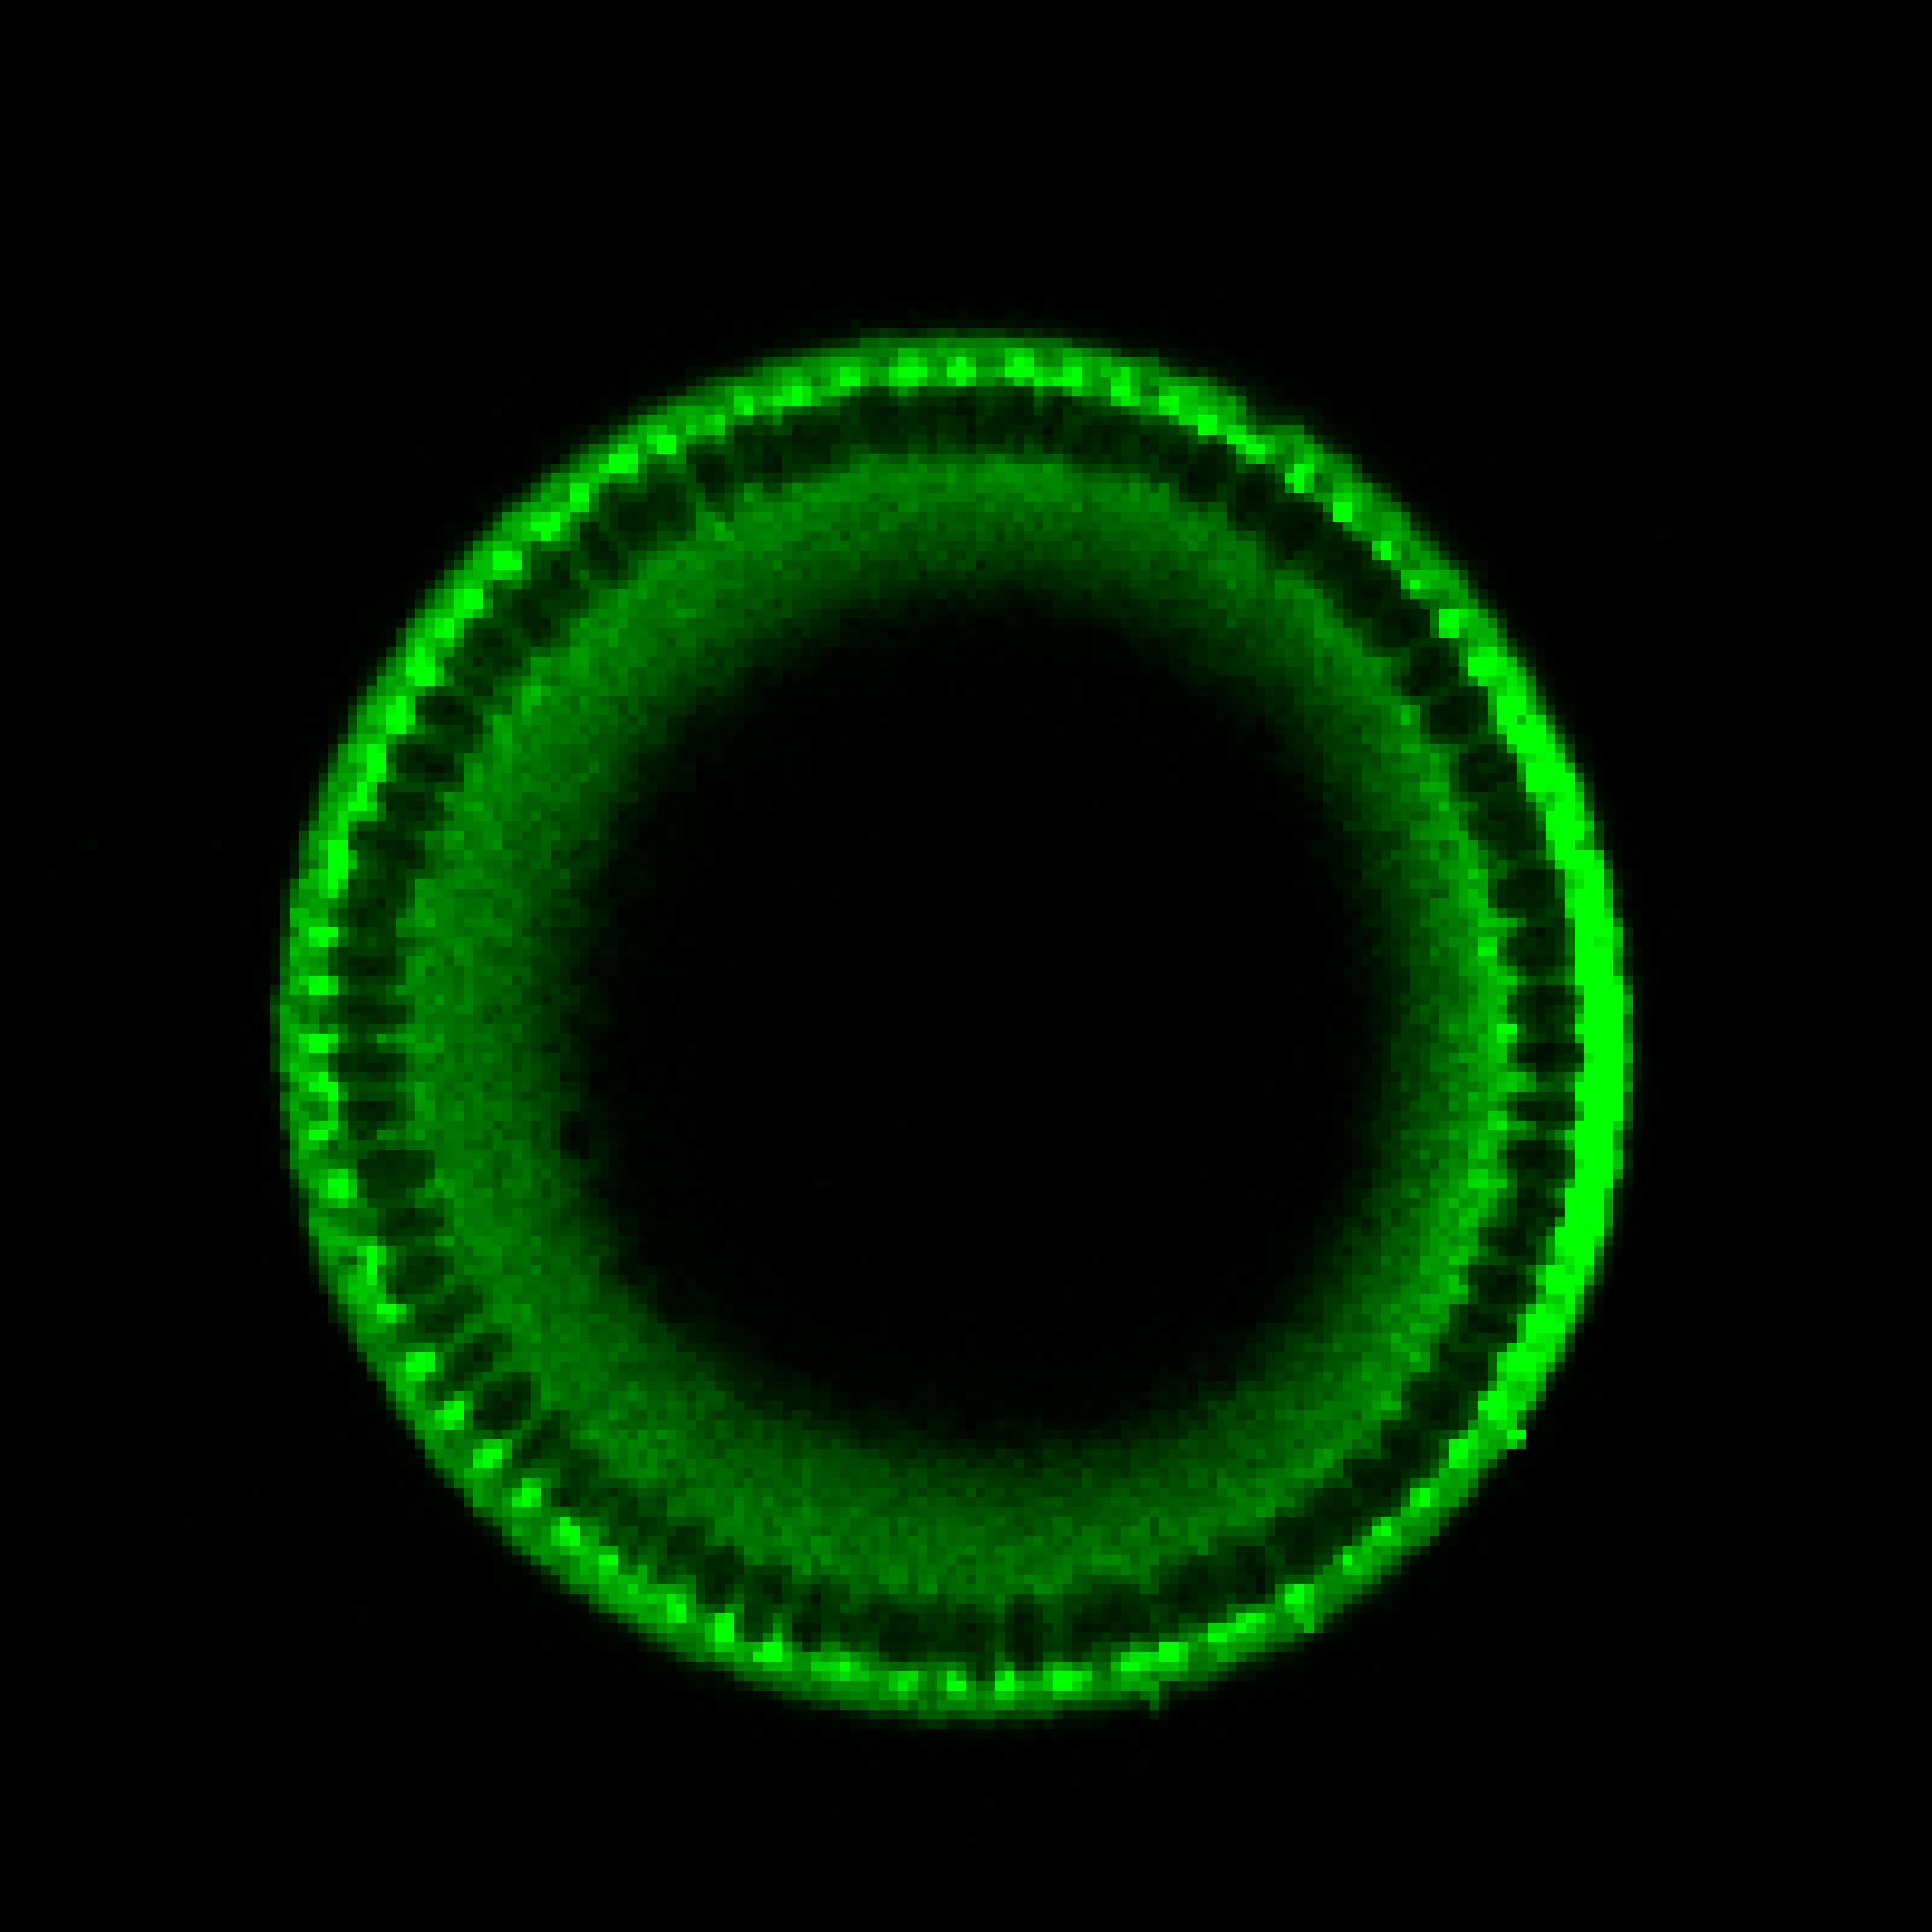
\includegraphics[width=0.1\textwidth]{membrane_scat_raw_1}};	
%    	\node[right=0.1in of fig3b](fig4b) {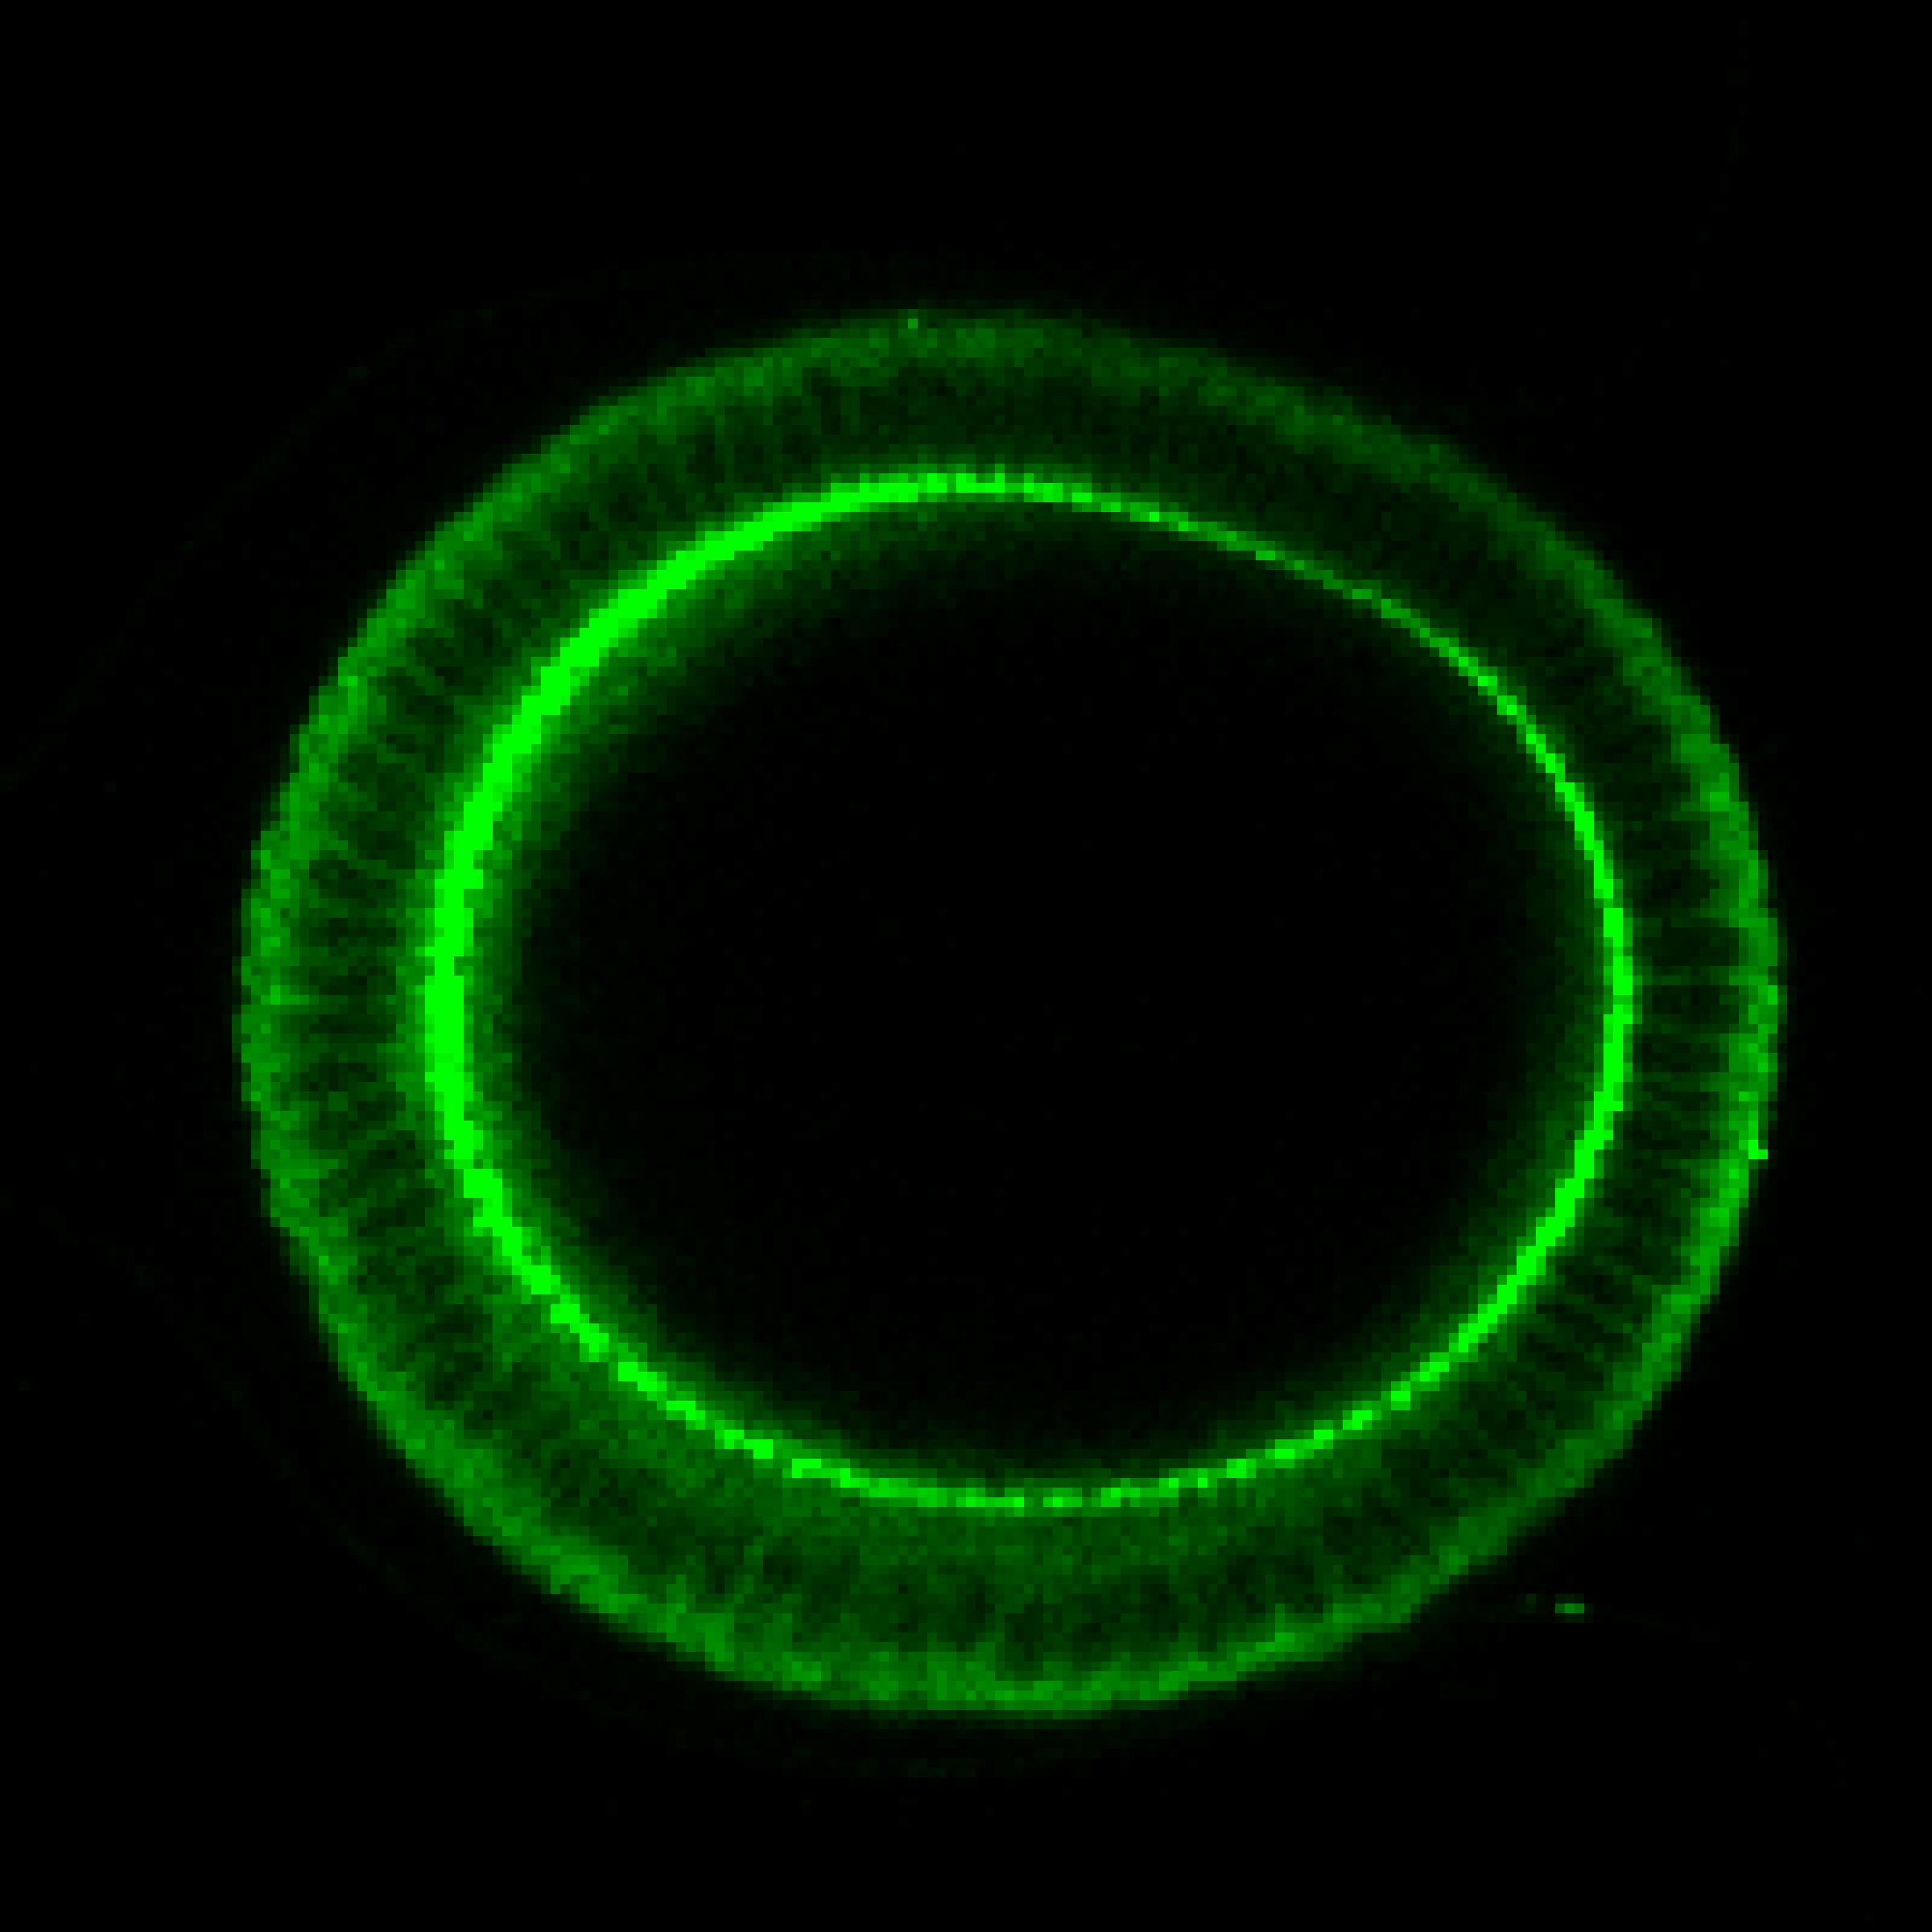
\includegraphics[width=0.1\textwidth]{membrane_scat_raw_4}};					
%    	\node[right=0.1in of fig4b](fig5b) {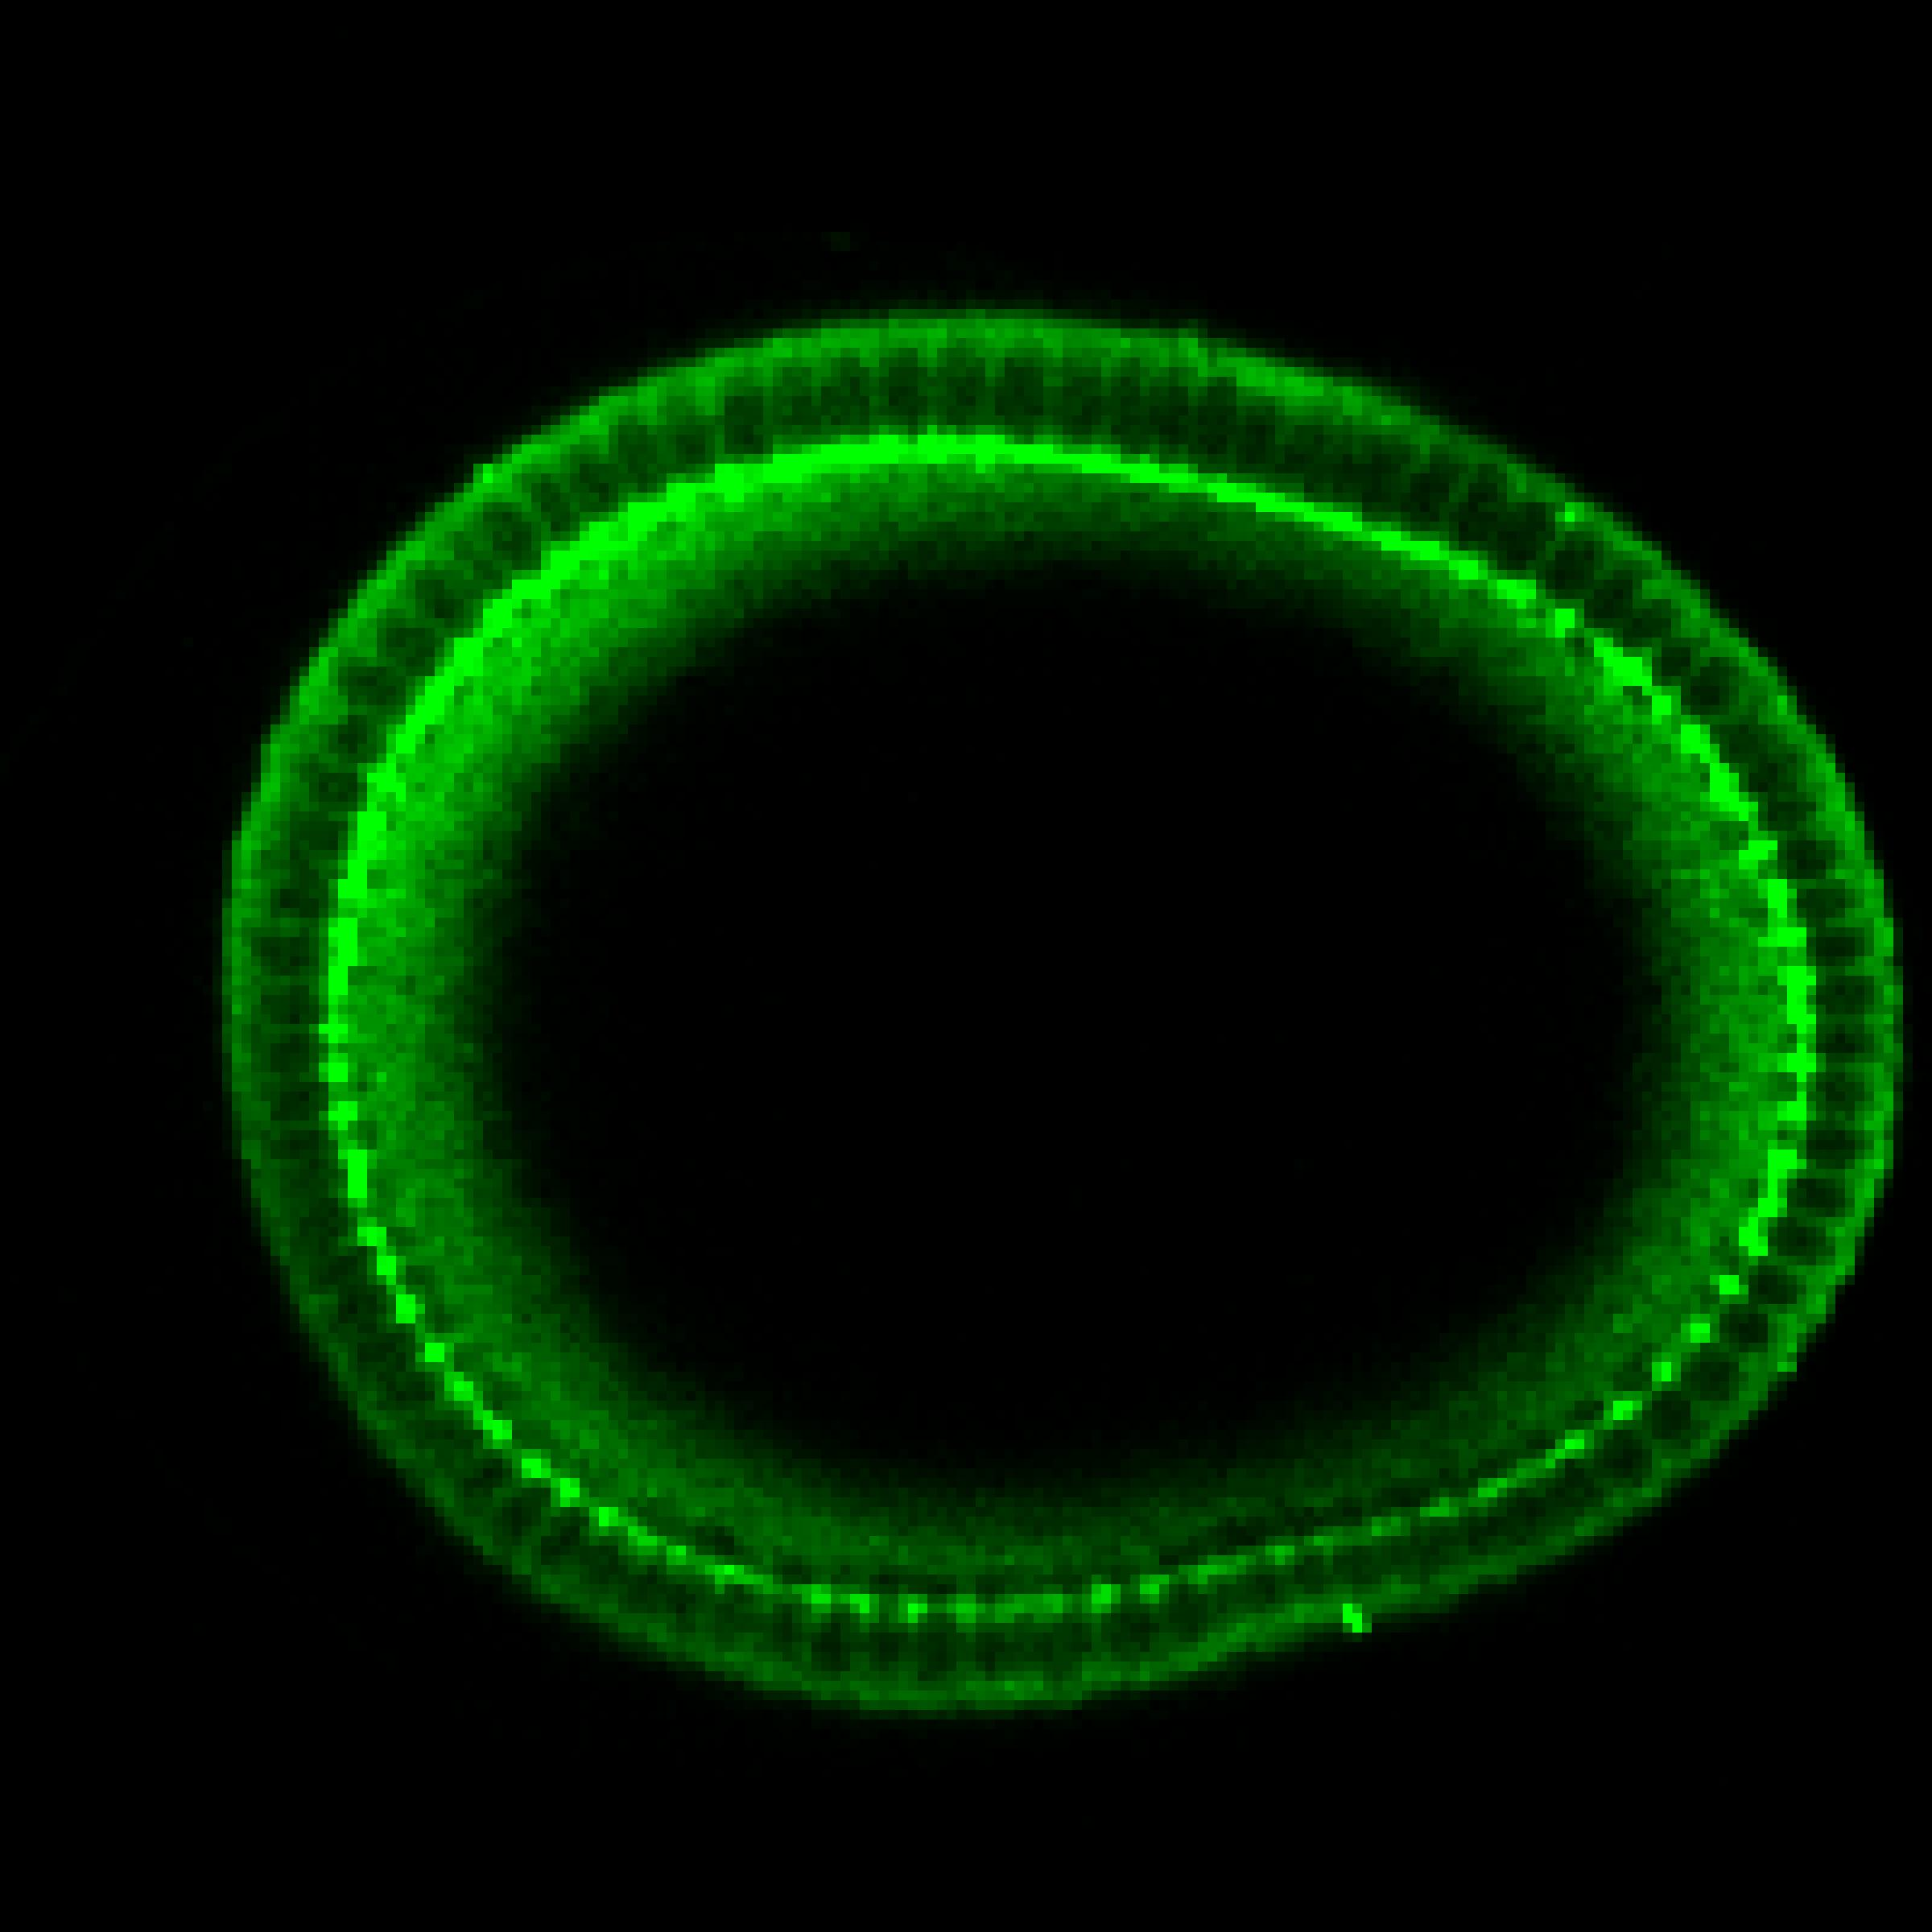
\includegraphics[width=0.1\textwidth]{membrane_scat_raw_5}};	    
%    	\draw[->] (x1) -- (fig1.north);
%    	\draw[->] (x2) -- (fig2.north);
%    	\draw[->] (x3) -- (fig3.north);
%    	\draw[->] (x4) -- (fig4.north);
%    	\draw[->] (x5) -- (fig5.north);
%    \end{tikzpicture}
%    
%    The first DMAPS coordinate is well-correlated with the membrane thickness.	
    
We then compute the scattering transform of the (edge--detected) images, and use this in a DMAPS calculation.

    \foreach \i in {15, 19, 30, 42, 45, 10, 36, 46, 47, 51, 27, 24, 28, 48, 38, 52, 34, 20, 50, 17, 6, 22, 16, 39, 33, 21, 2, 41, 9, 29, 14, 4, 8, 35, 31, 3, 40, 44, 13, 7, 18, 32, 11, 43, 25, 49, 5, 26, 23, 37, 12} {	
	\includegraphics[width=0.05\textwidth]{membrane_scat_all_\i}} 
    
    	\centering
    {\Large $\downarrow$}
    
	\foreach \i in {2,...,52} {
	\includegraphics[width=0.05\textwidth]{membrane_scat_all_\i}
	}   


\end{frame}

    
    

    